\chapter{動作検証}
\label{chp:tex_pro}
この章では動作検証の結果をスクリーンショットとソースコードを元に紹介する.
今回はGoogle Chrome上で動作させるため,他のWebブラウザ上ではUIが異なっている可能性がある.

\section{社員が写真を提出する}
\label{sec:tex_pro_cmd}
社員ページに顔写真提出するためのフォームを作成した.写真提出ボタンから提出する写真を選択し,
提出する.その実行しているスクリーンショットを図4.1,図4.2,図4.3,図4.4に示す.

もし顔認識できない写真であれば,もう一度写真を提出させる処理をすることでエラー回避している
(ソースコード4.1).そのスクリーンショットを図4.5に示す.

\begin{lstlisting}[caption=顔認識エラー処理]
  if (object.length !== undefined) {
    return (
      <div>
        <p>顔認識できません。</p>
        <p
          className="submit reset"
          onClick={() => {
            setNum(1);
          }}
        >
          やり直す
        </p>
      </div>
    );
  }
\end{lstlisting}

\vspace{4mm}

\begin{figure}[!h]
	\begin{center}
			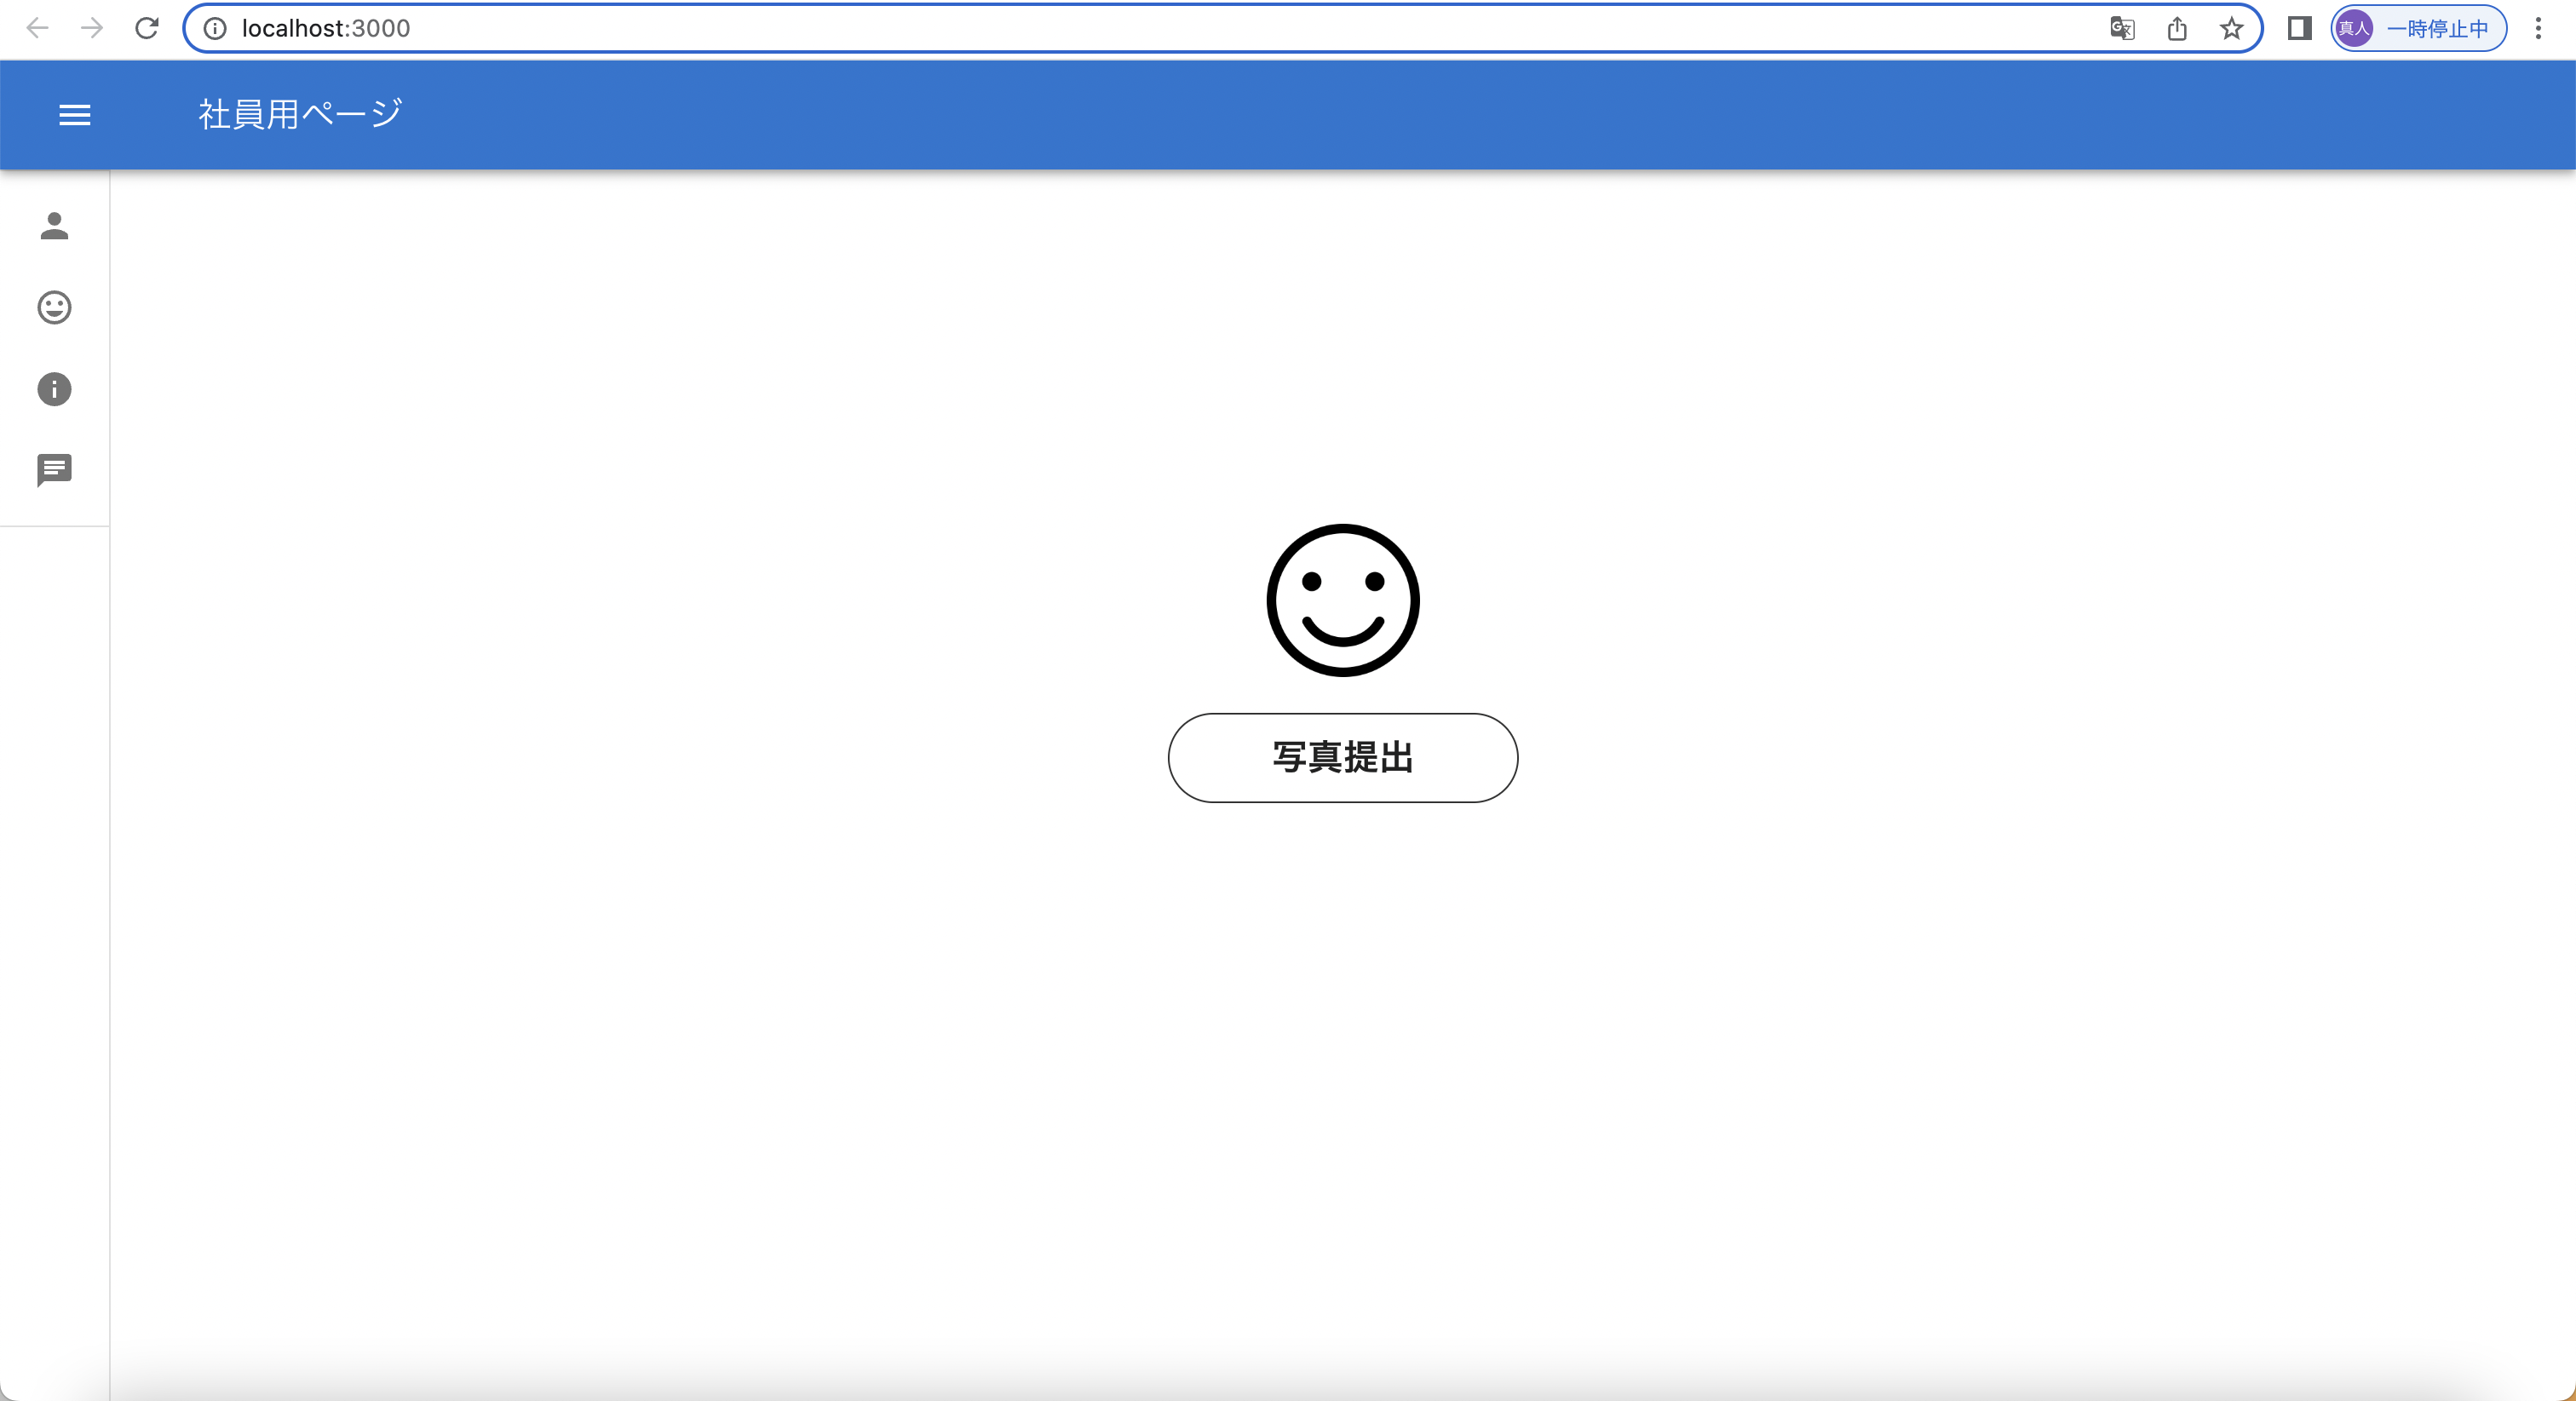
\includegraphics[scale=0.3, clip]{./img/sample1.png}
			\caption{提出画面}
			\label{fig:図の名前}
	\end{center}
\end{figure}

\begin{figure}[!h]
	\begin{center}
			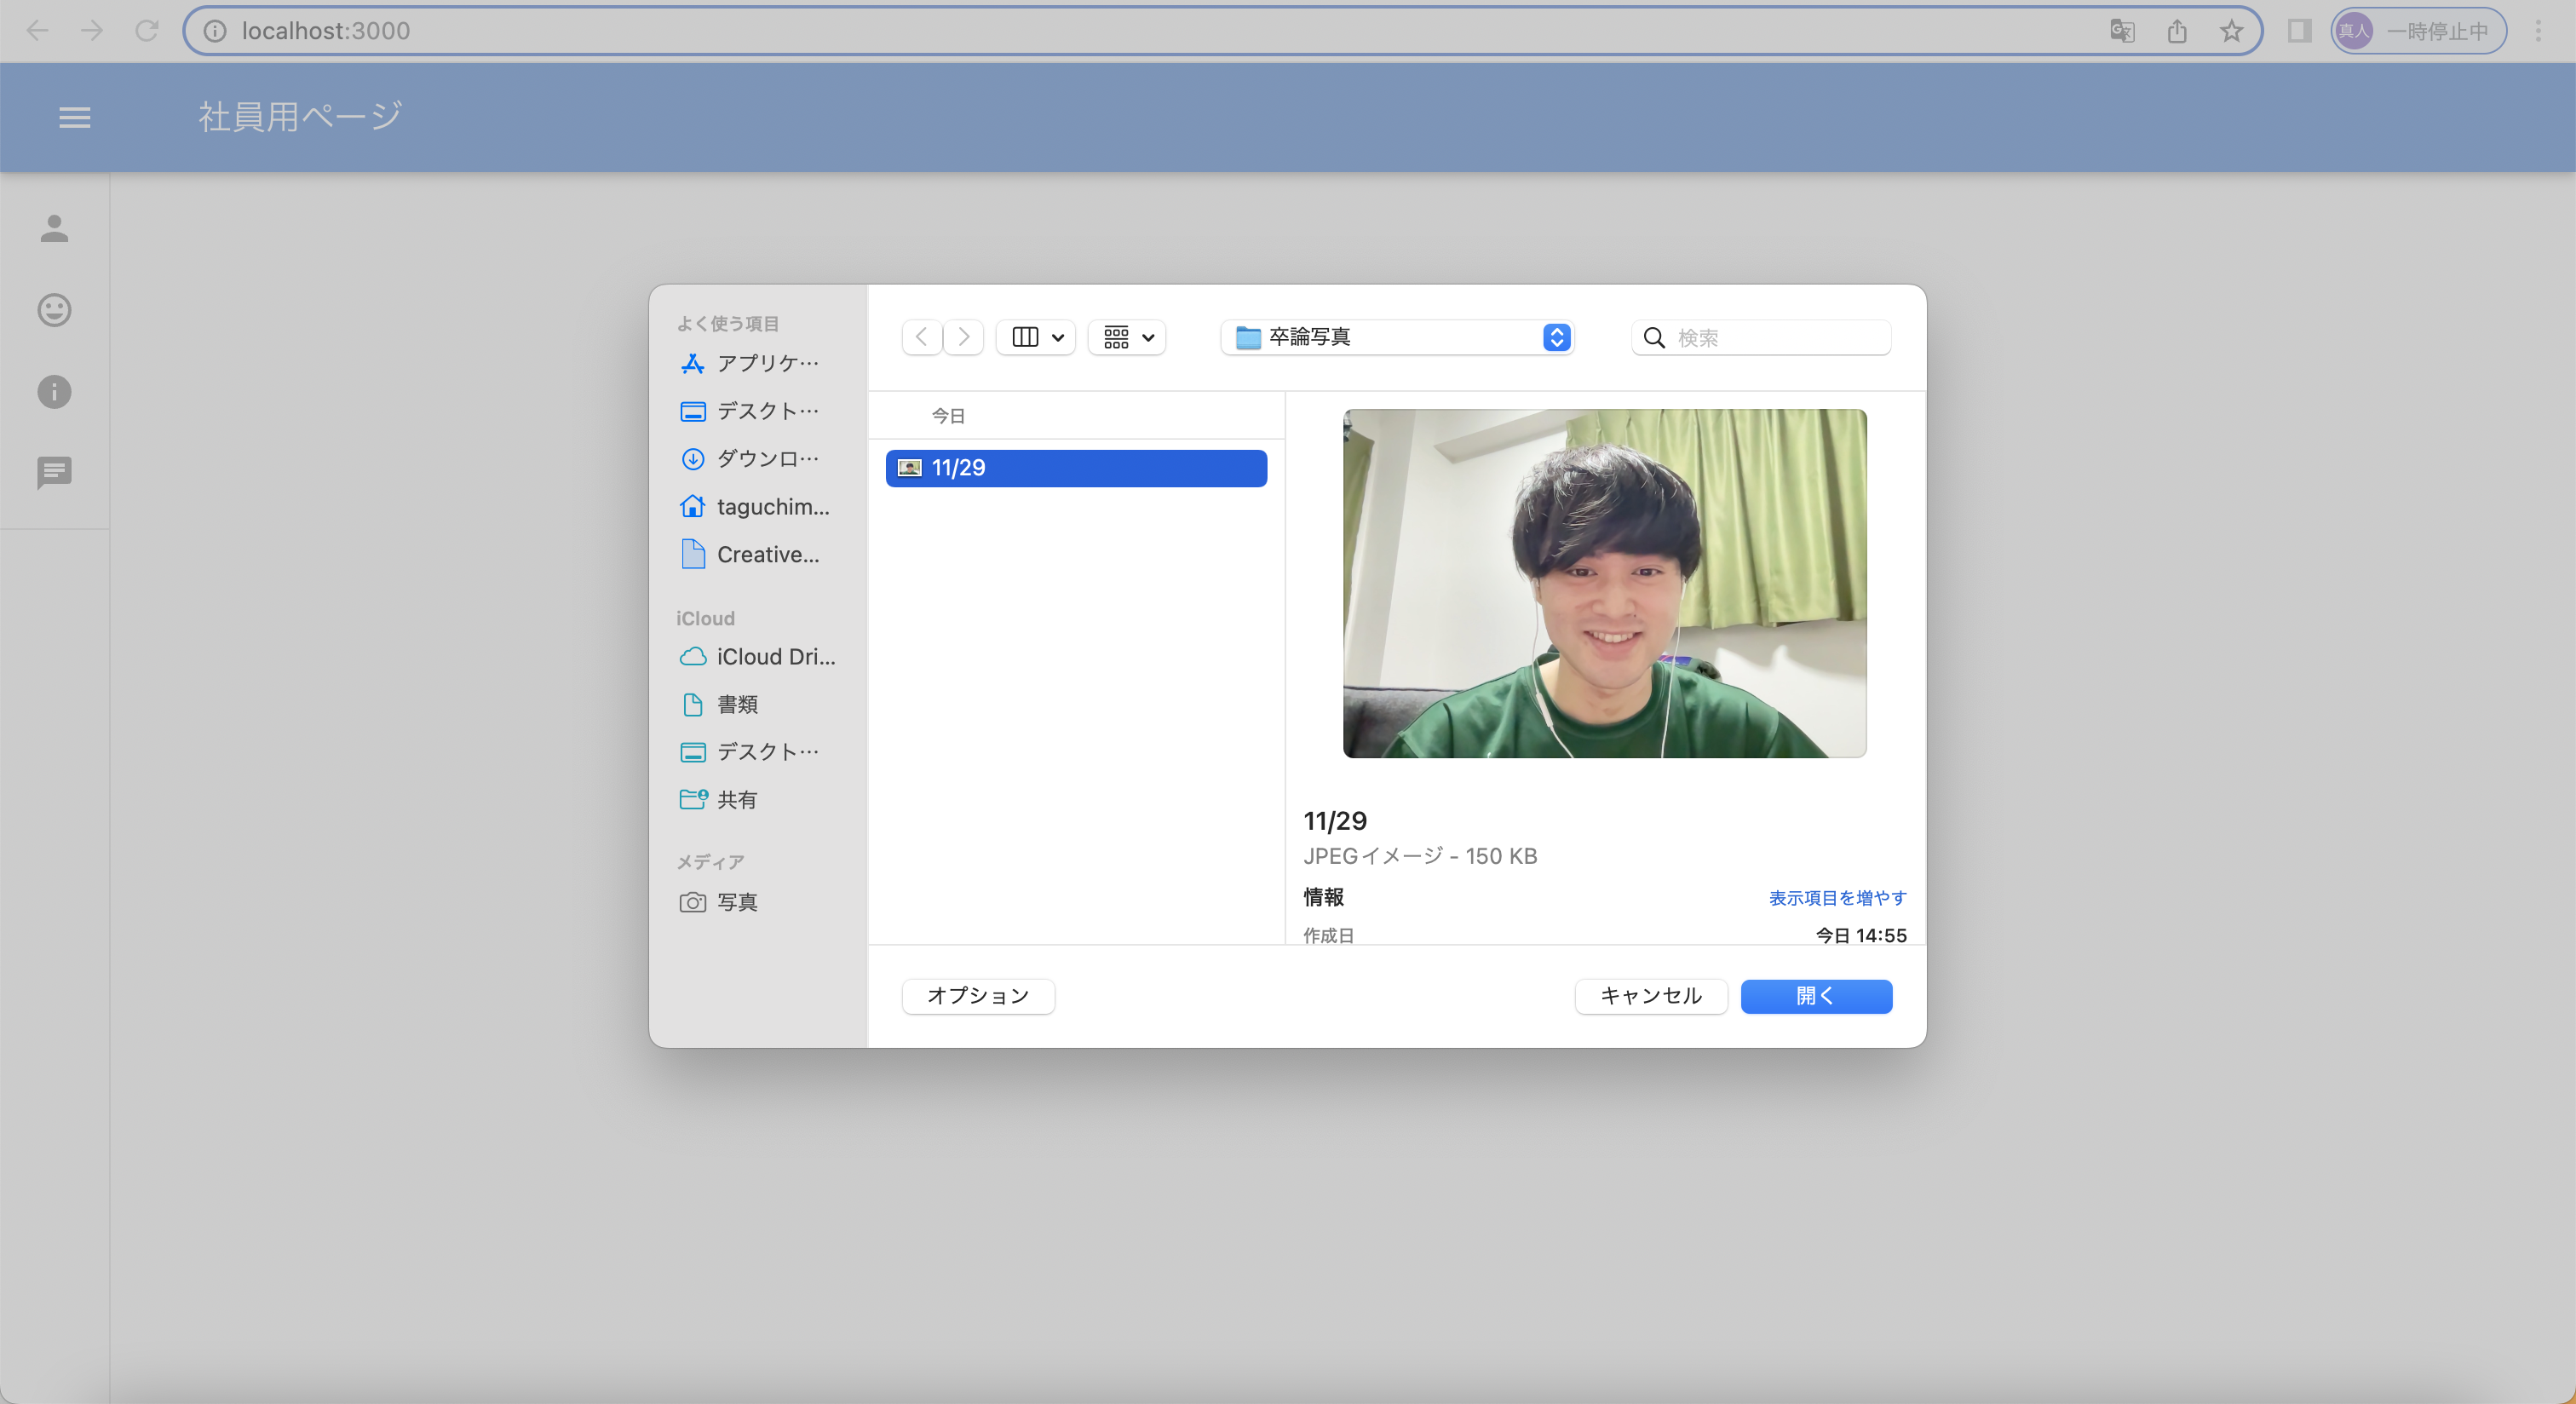
\includegraphics[scale=0.3, clip]{./img/sample2.png}
			\caption{写真選択画面}
			\label{fig:図の名前}
	\end{center}
\end{figure}

\begin{figure}[!h]
	\begin{center}
			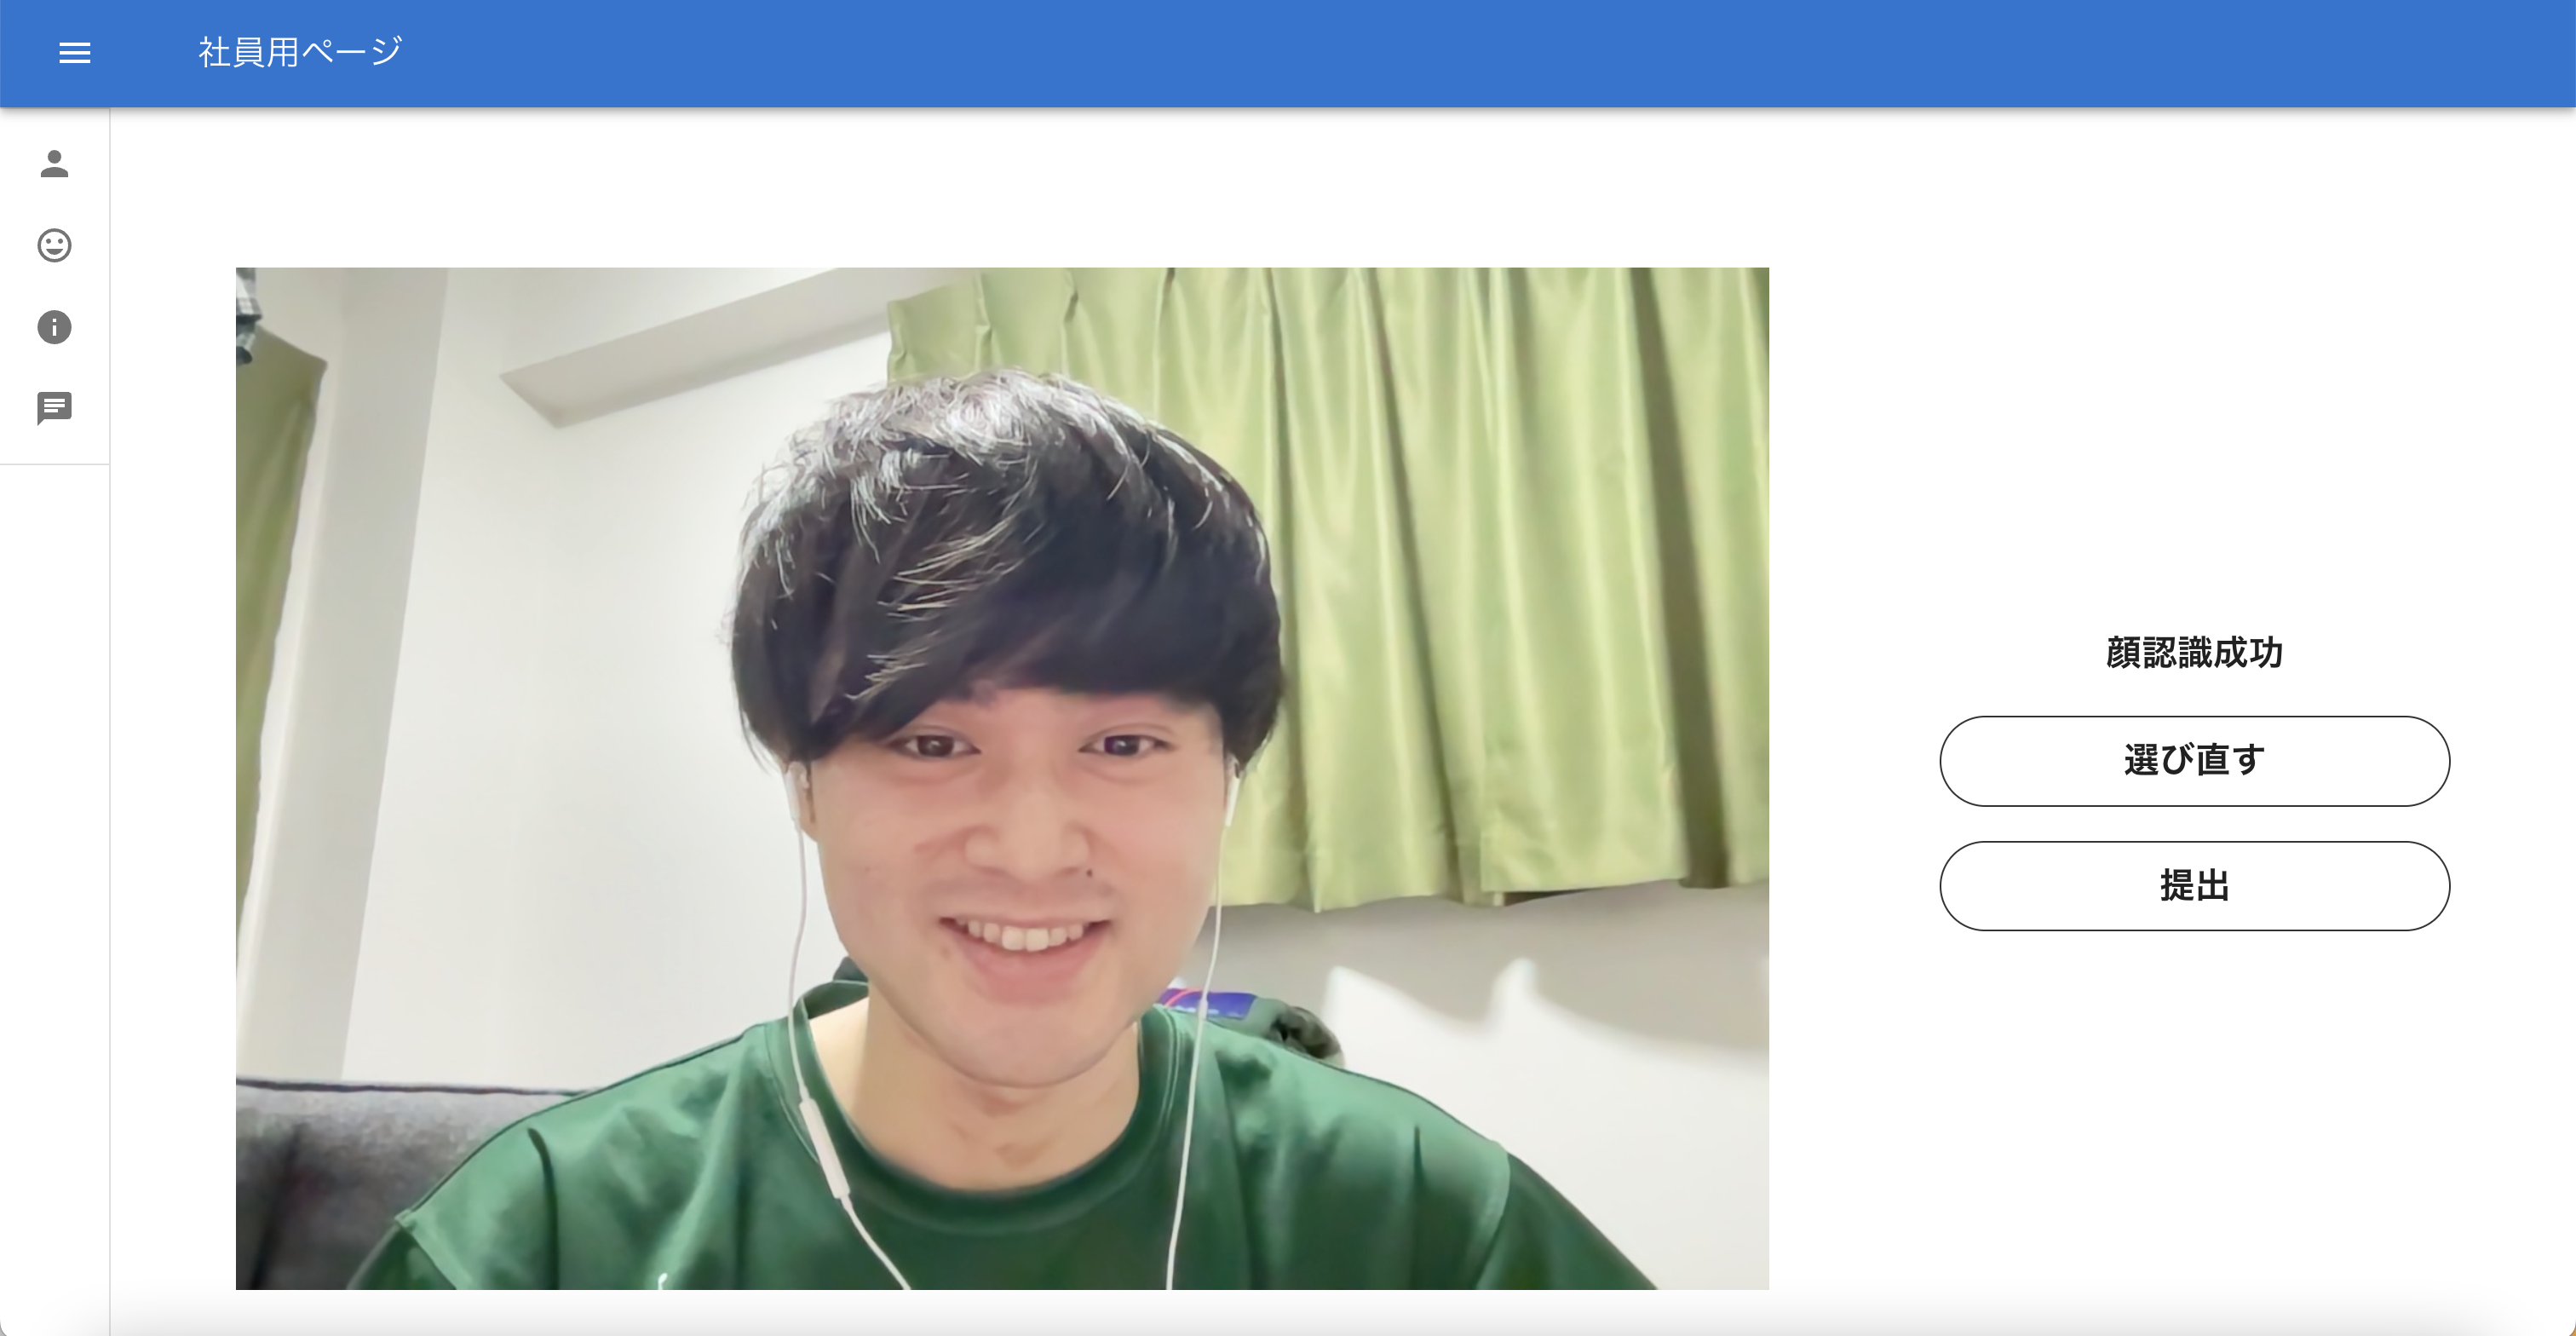
\includegraphics[scale=0.3, clip]{./img/sample3.png}
			\caption{画面}
			\label{fig:図の名前}
	\end{center}
\end{figure}

\begin{figure}[!h]
	\begin{center}
			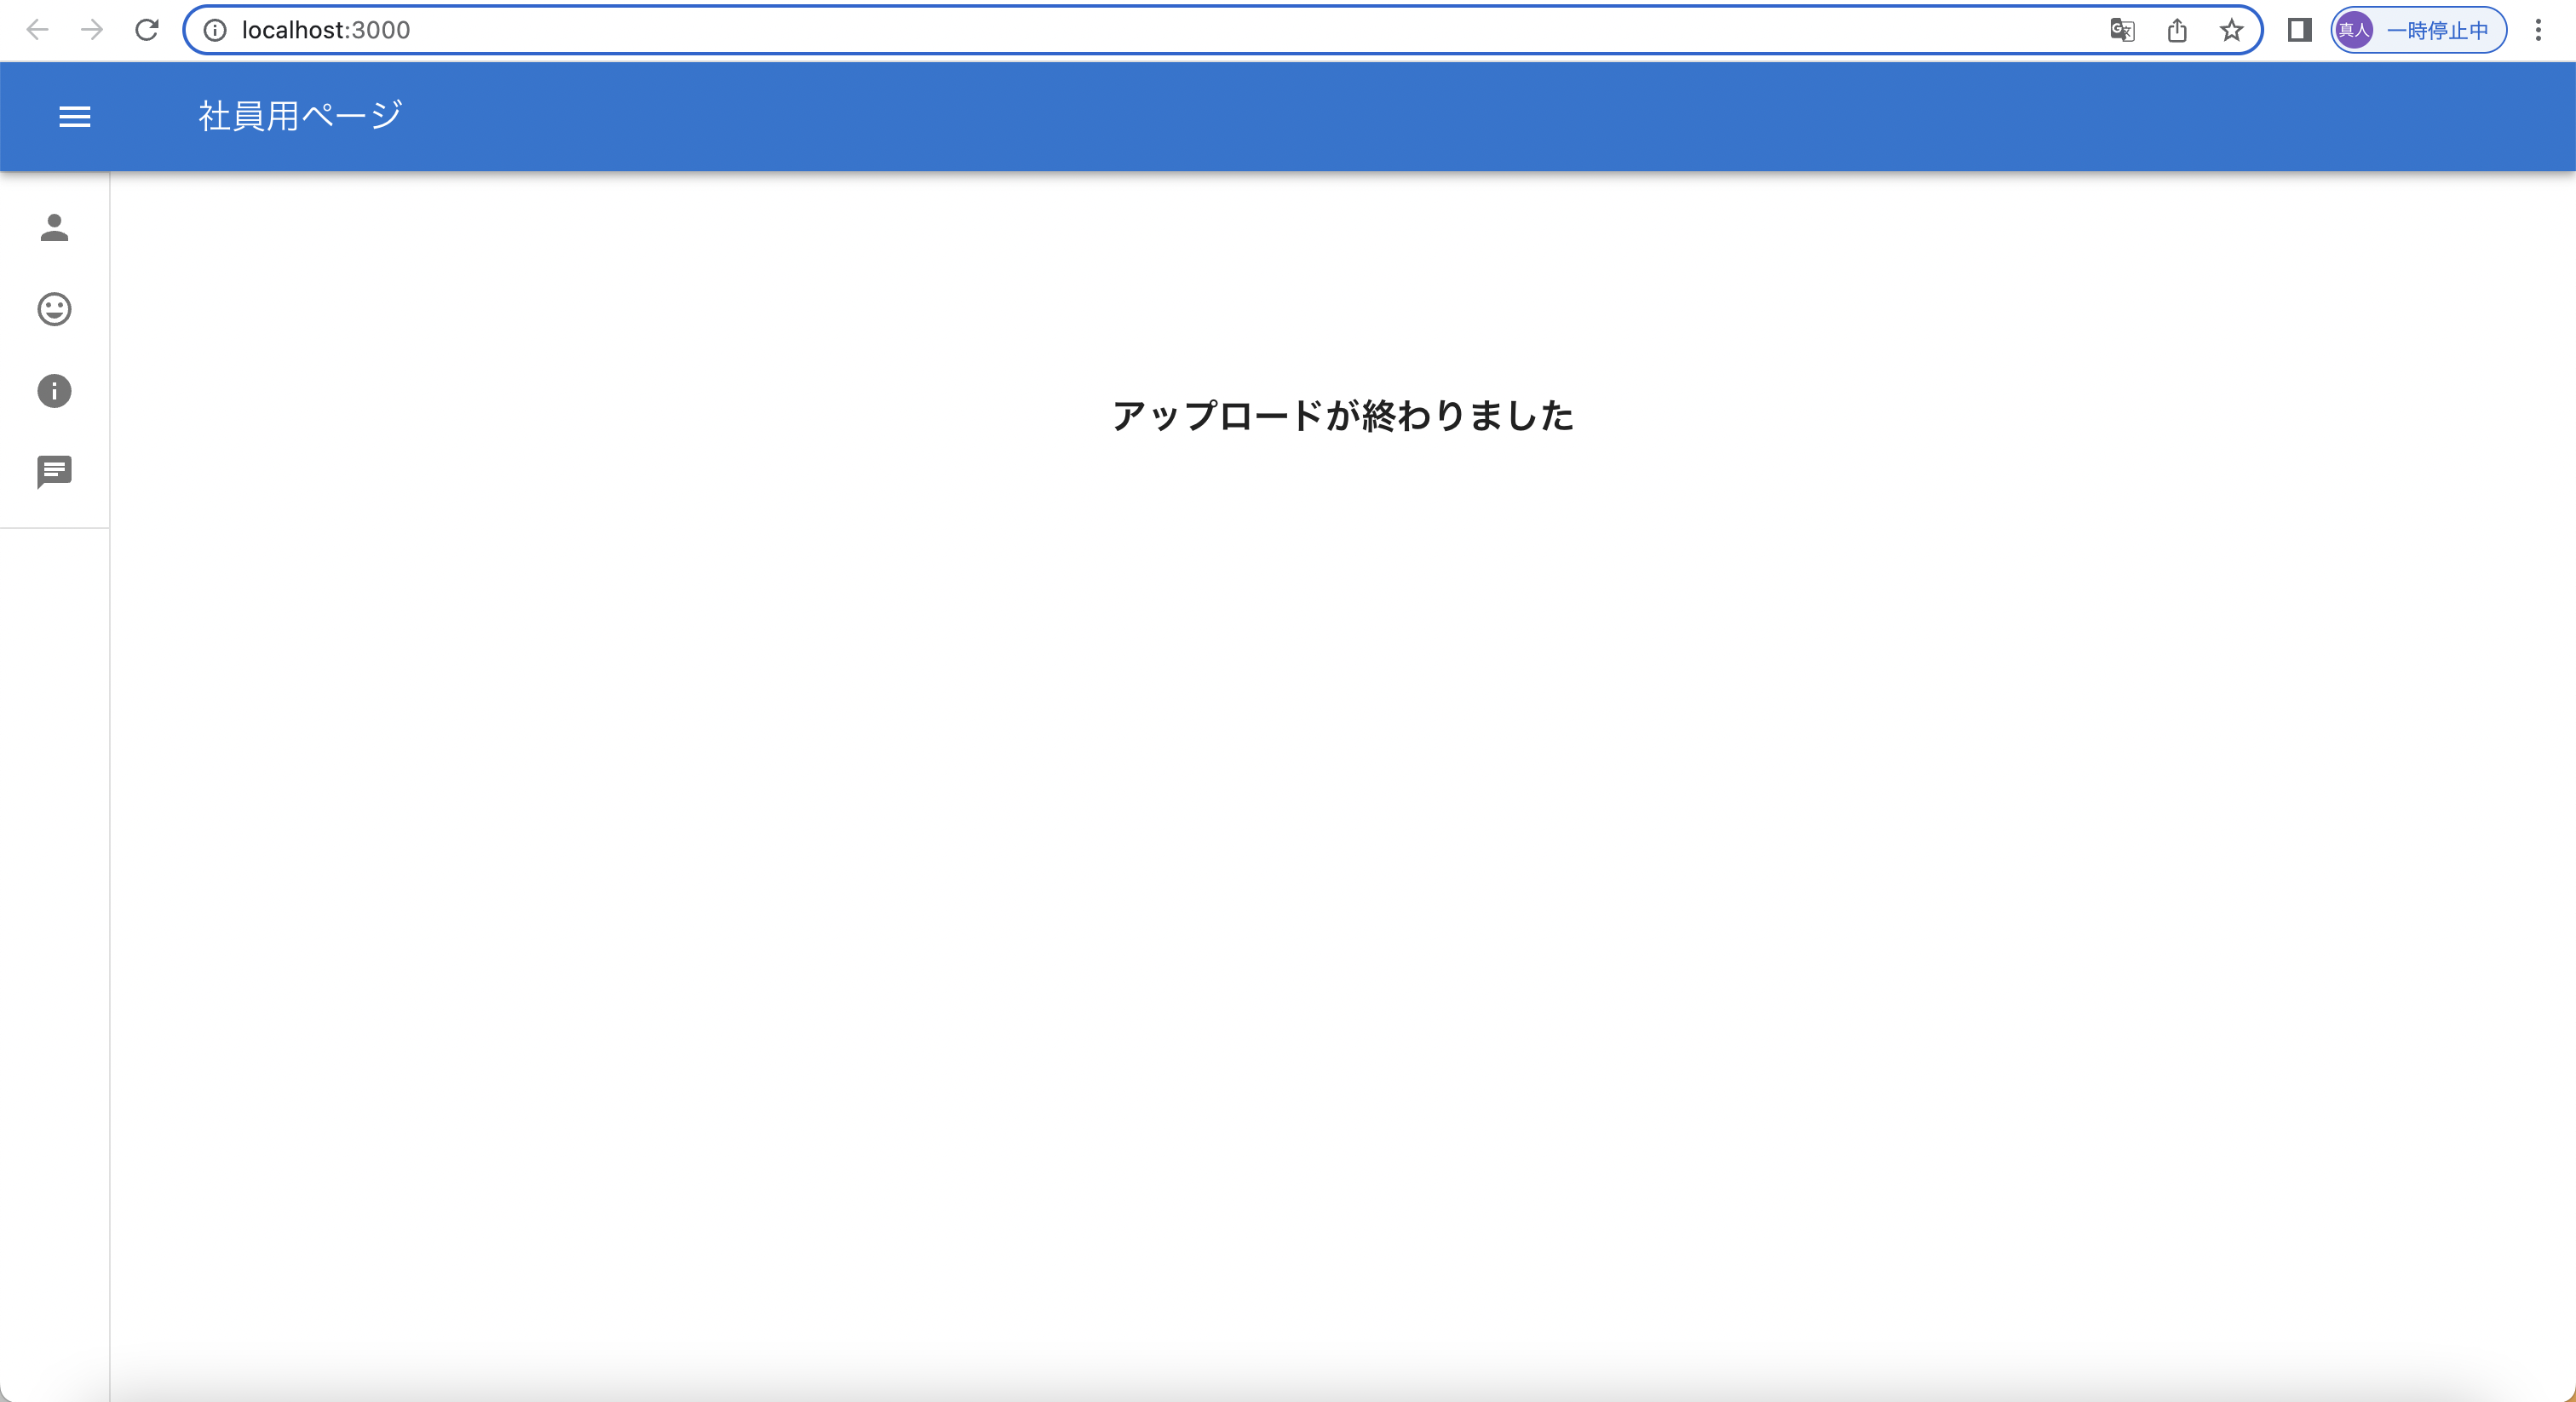
\includegraphics[scale=0.3, clip]{./img/sample4.png}
			\caption{提出完了画面}
			\label{fig:図の名前}
	\end{center}
\end{figure}

\clearpage

\begin{figure}[!h]
	\begin{center}
			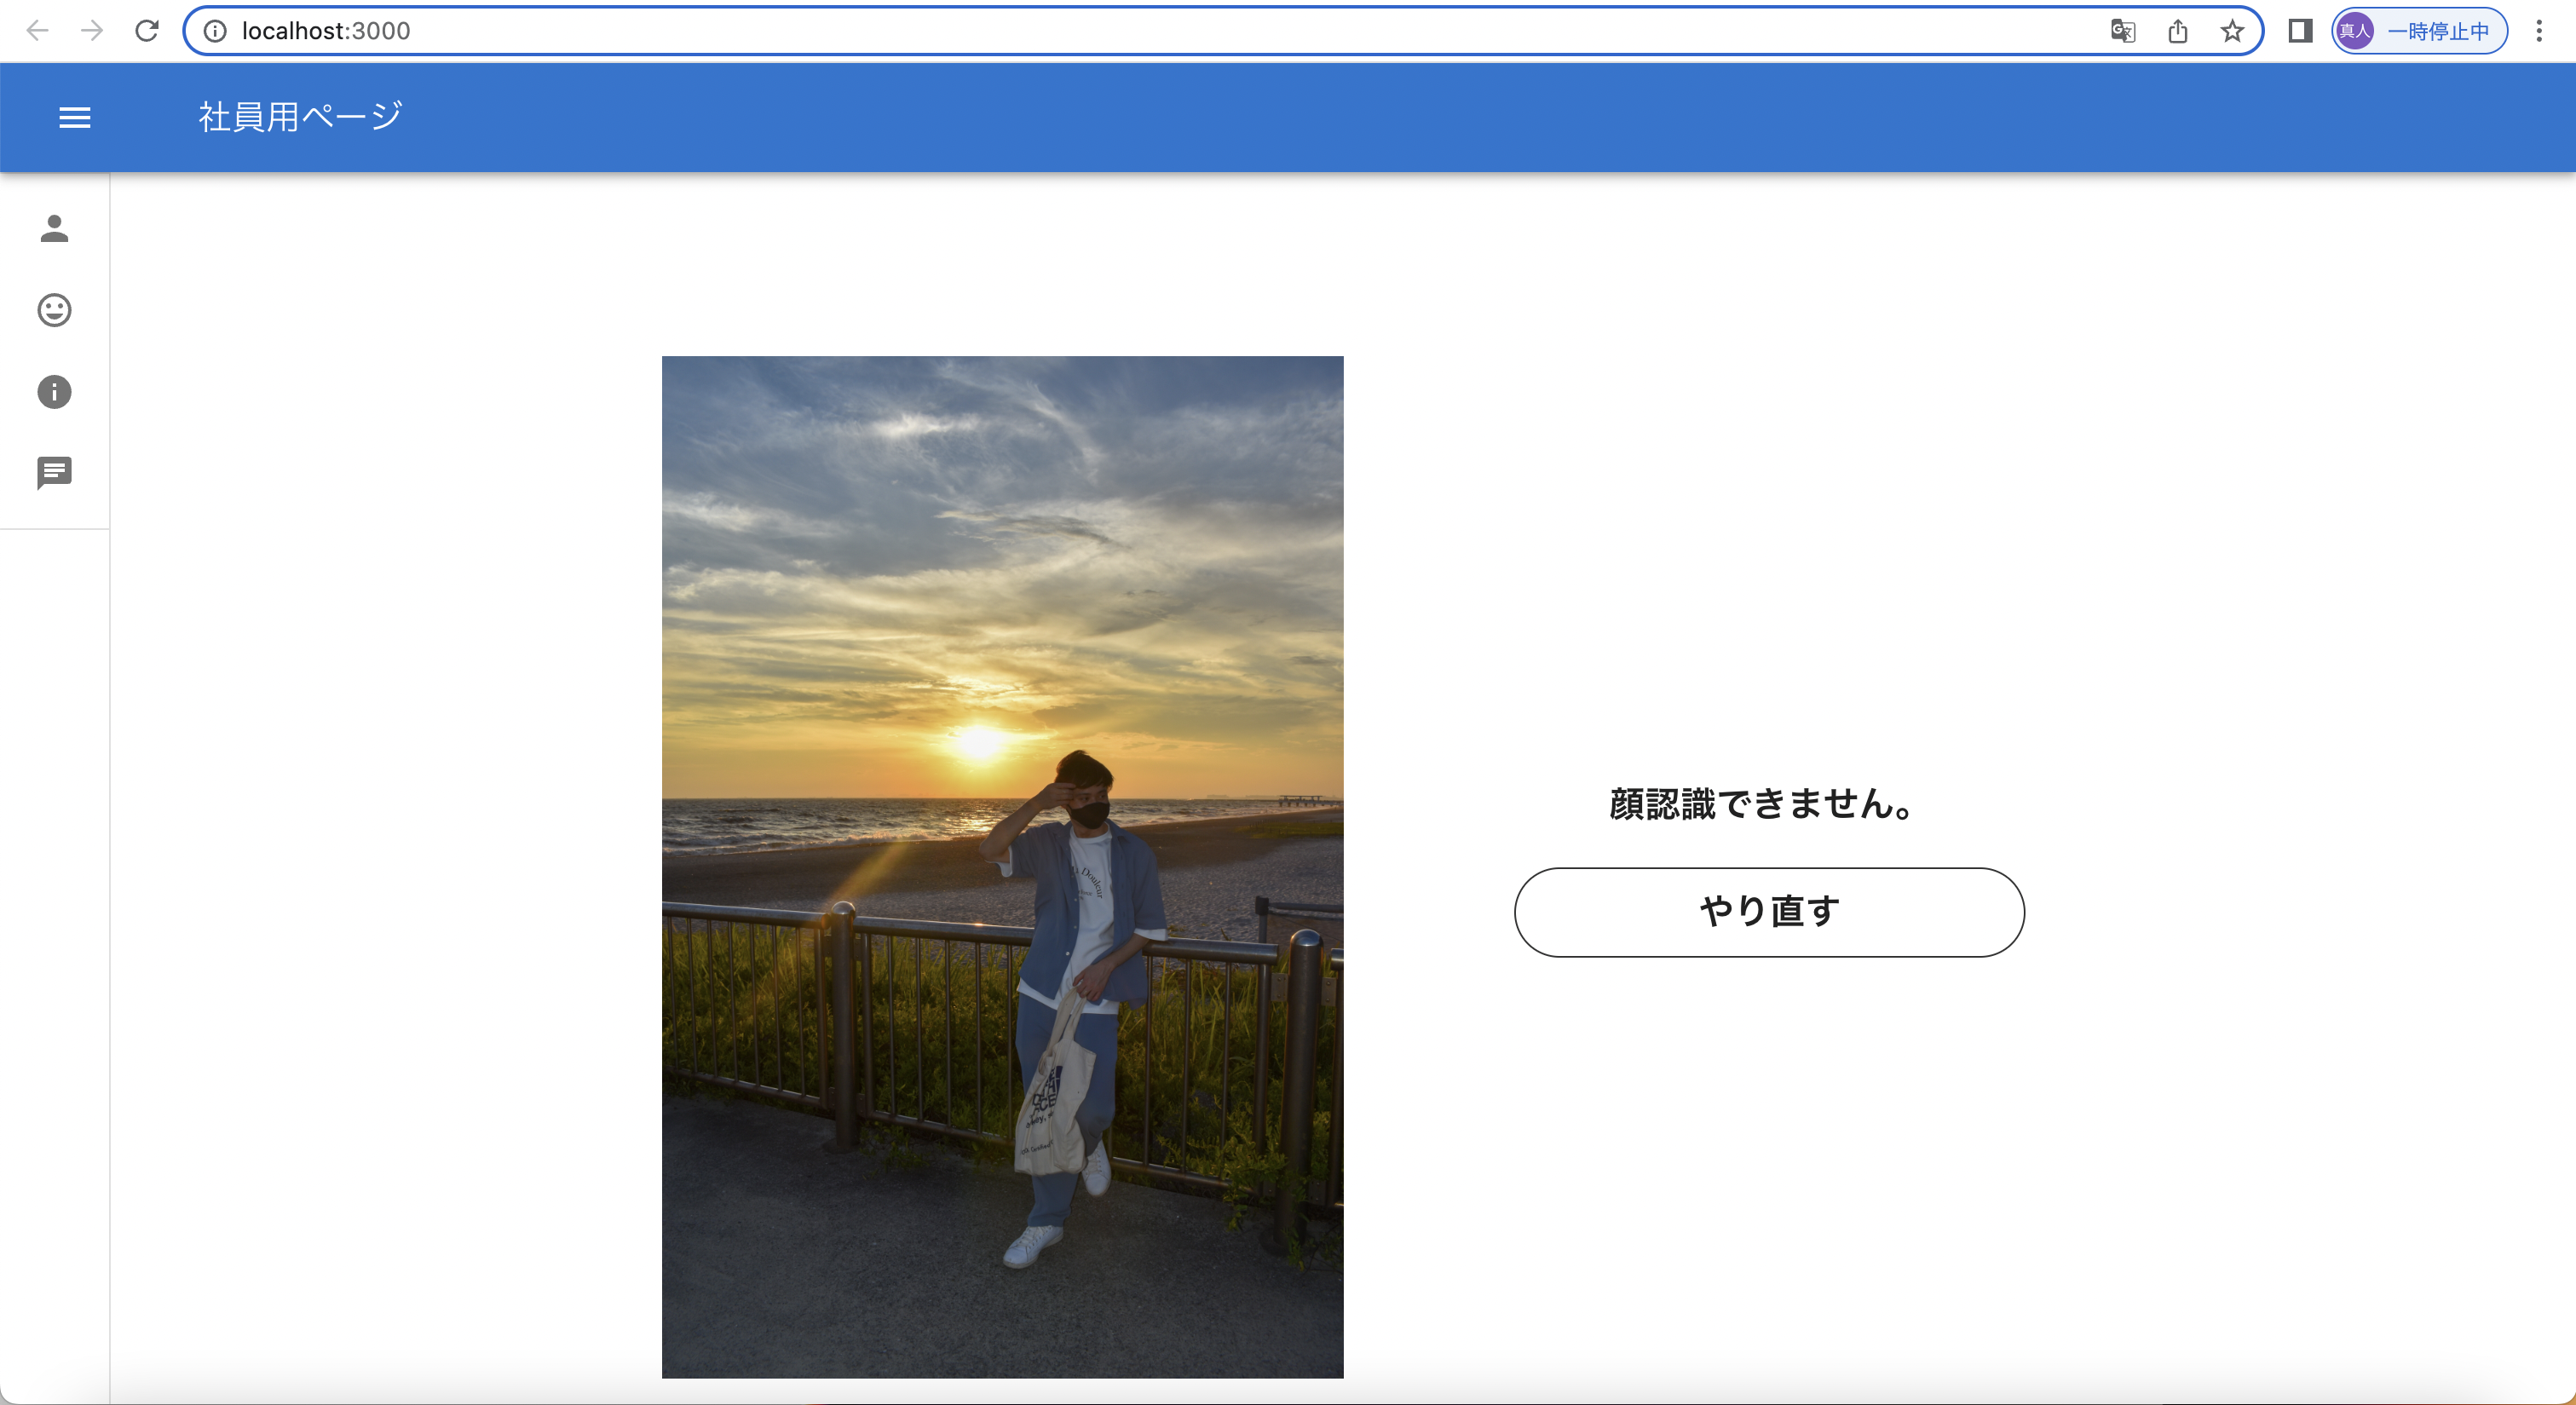
\includegraphics[scale=0.3, clip]{./img/sample5.png}
			\caption{顔認識失敗画面}
			\label{fig:図の名前}
	\end{center}
\end{figure}

\section{管理者の社員管理機能}
\label{chp:tex_admin}
管理者ページでは,管理者が社員を管理しやすくするために,表で管理しており,
社員ID,名前,メールアドレス,笑みポイントを可視化している.
図4.6に表が表示されているスクリーンショットを示す.
その他に,それぞれの社員の名前やメールアドレスなどを編集できる機能,提出された写真を見る機能,
社員とトークできる機能がある.それぞれについて,以下で説明する.

\subsection{編集機能}
編集ページのスクリーンショットを図4.7に示す.
編集機能では,社員ID,笑みポイント,役職,名前,メールアドレスを編集できる.
編集した社員IDが他の社員IDと被ってしまうとエラーが起きてしまうので,ソースコード4.2,
ソースコード4.3の様にしてエラー回避している.変数querySnapshot2でidが被っているユーザーを
検索し,変数qに配列として代入している.idが一つでも被っていたらqの大きさは0では無くなるので,
ソースコード4.2の9行目から始まるif文とソースコード4.3でidが被った際の処理をしている.
その際のスクリーンショットを図4.8に示す.

\clearpage

\begin{lstlisting}[caption=社員IDが被った時の処理]
  const handleSubmit = async (event) => {
    event.preventDefault();
    const data = new FormData(event.currentTarget);
    const id = Number(data.get("id"));
    const querySnapshot2 = await getDocs(
      query(collection(db, "users"), where("id", "==", id)));
    const q = querySnapshot2.docs.map((doc) => doc.id);

    if (q.length === 0) {
      setNum(2);
      // db更新
      const querySnapshot = await getDocs(
        query(collection(db, "users"), where("id", "==", props.count))
      );
      const docId = querySnapshot.docs.map((doc) => doc.id).toString();
      await updateDoc(doc(db, "users", docId), {
        id: Number(data.get("id")),
        name: data.get("name"),
        email: data.get("email"),
        point: Number(data.get("point")),
        role: data.get("role"),
      });
    } else {
      setNum(3);
    }
  };
\end{lstlisting}

\begin{lstlisting}[caption=社員IDが被った時の処理]
  else if (num === 3) {
    return (
      <div>
        <ArrowBackRoundedIcon
          sx={{ fontSize: 60 }}
          className="back"
          onClick={() => {setNum(0);}}
        />
        <p>idが被っています</p>
      </div>
    );
  }
\end{lstlisting}

\begin{figure}[!h]
	\begin{center}
			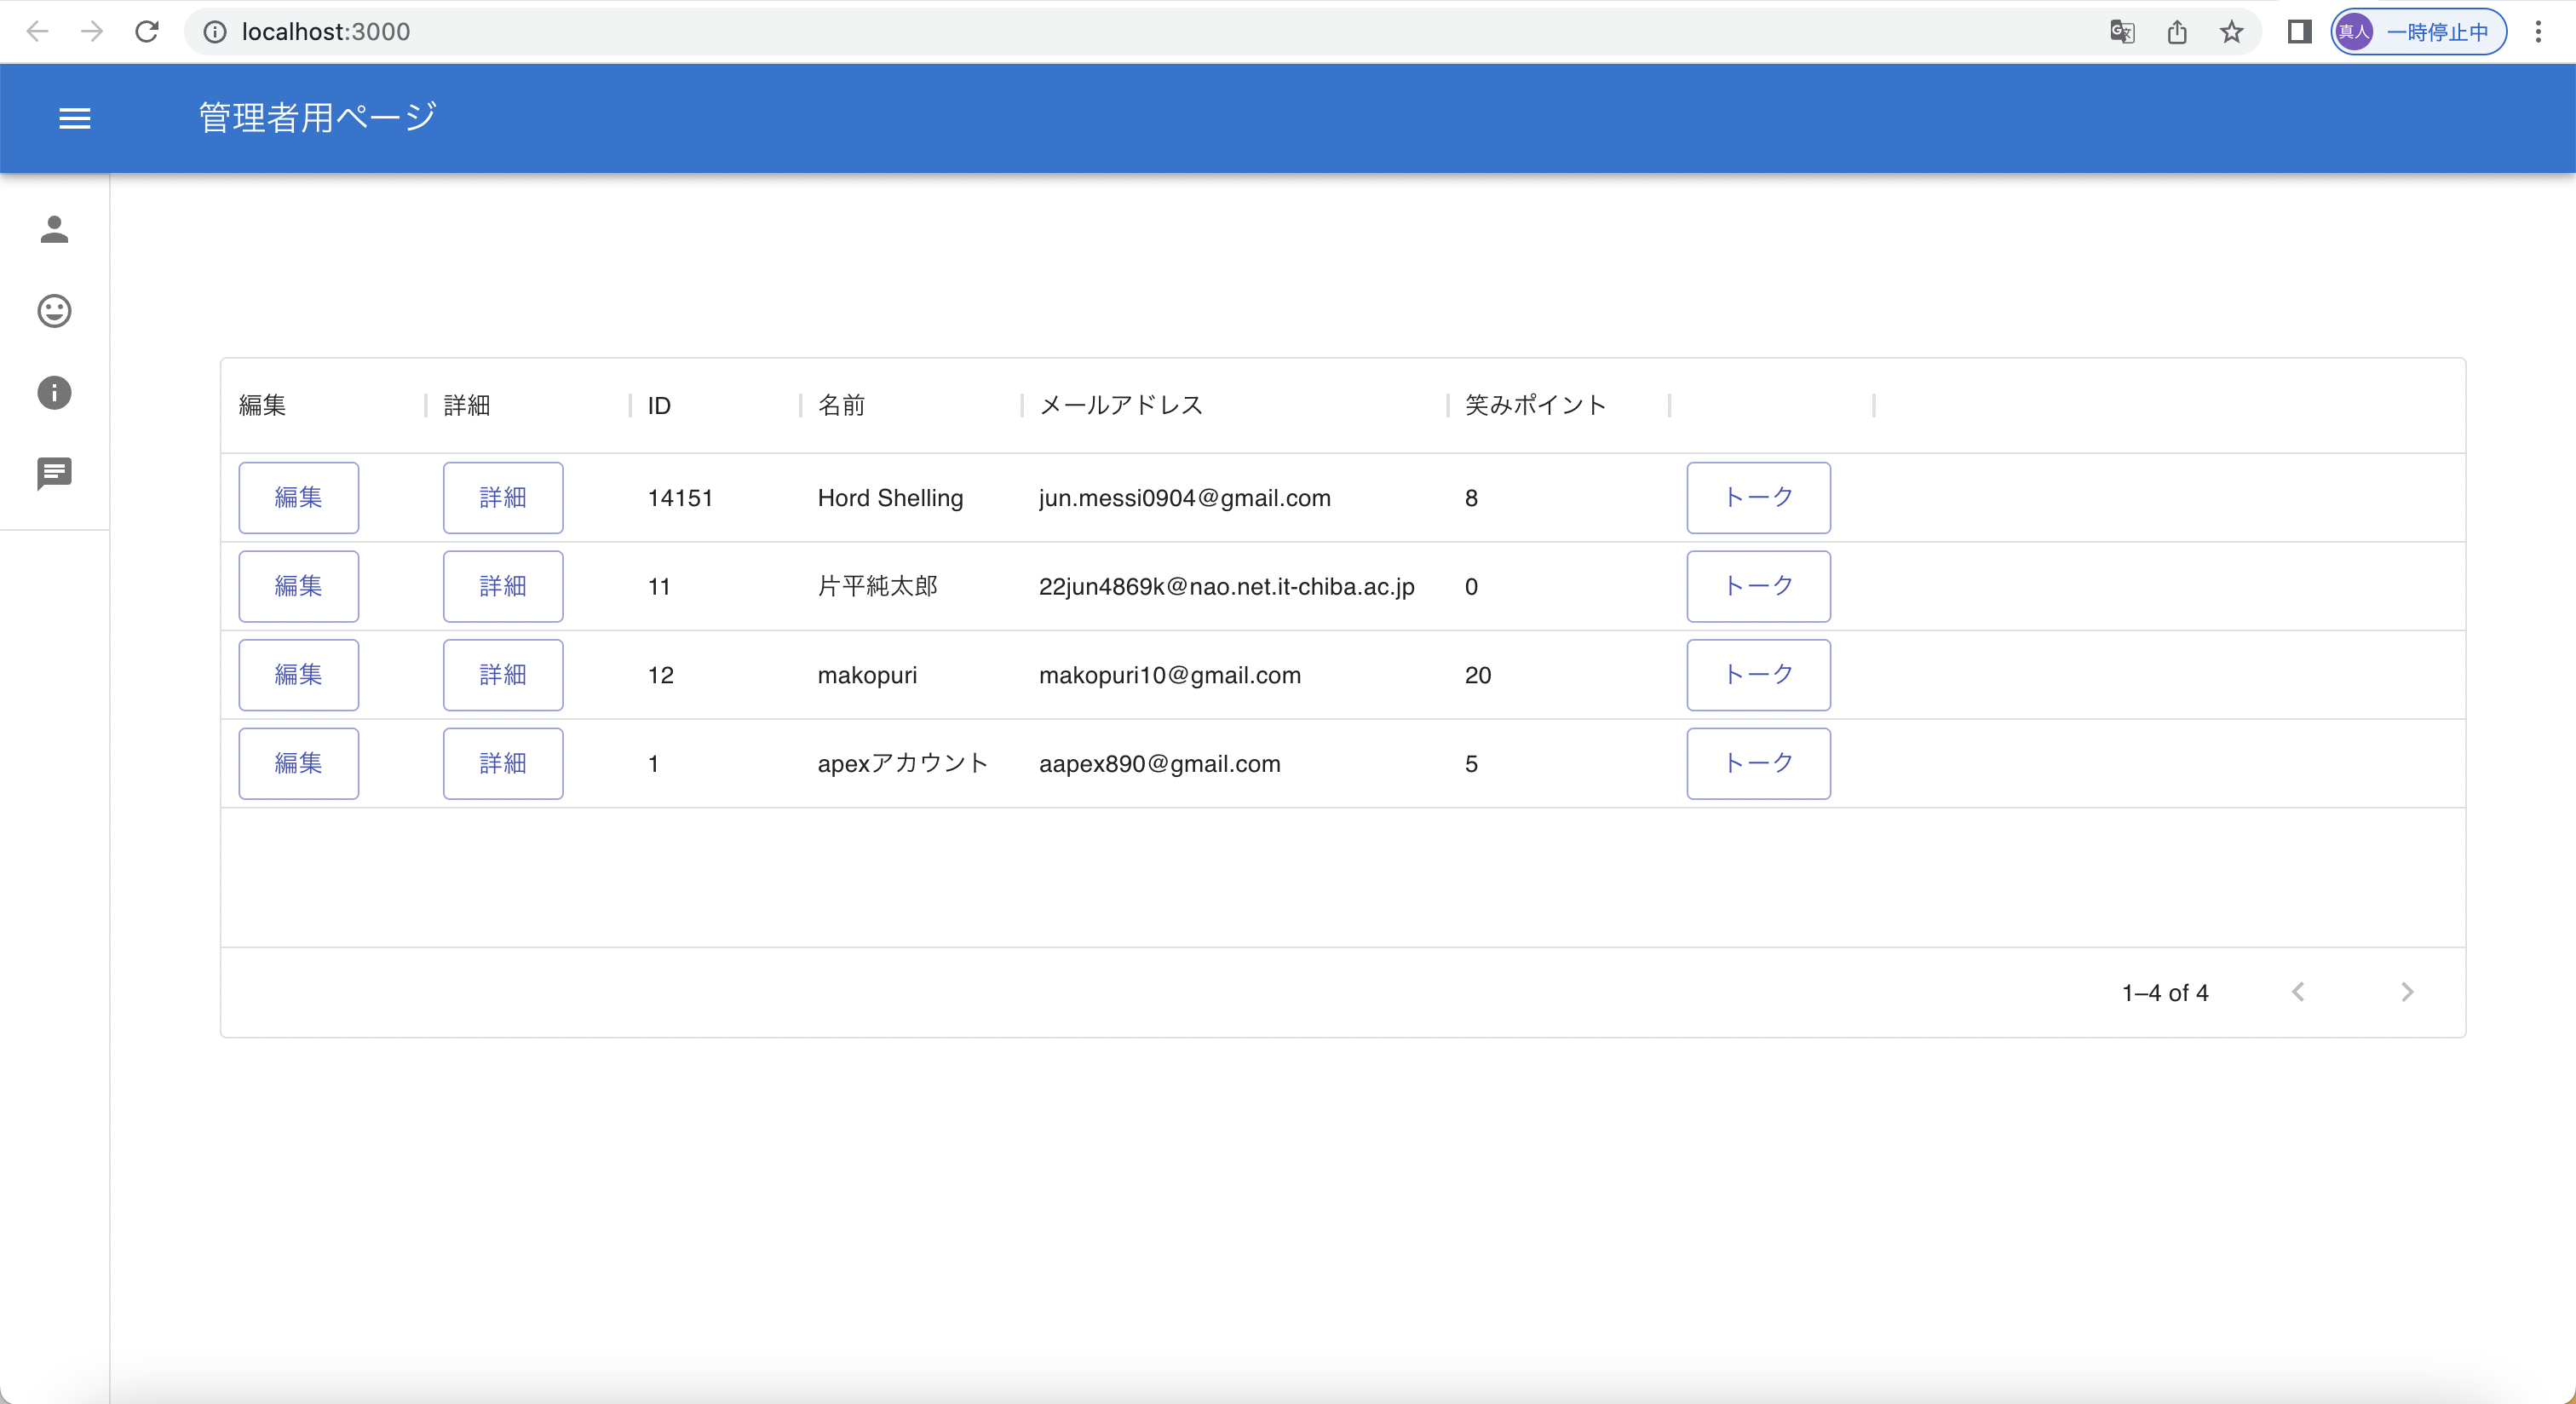
\includegraphics[scale=0.3, clip]{./img/sample6.png}
			\caption{社員管理画面}
			\label{fig:図の名前}
	\end{center}
\end{figure}

\begin{figure}[!h]
	\begin{center}
			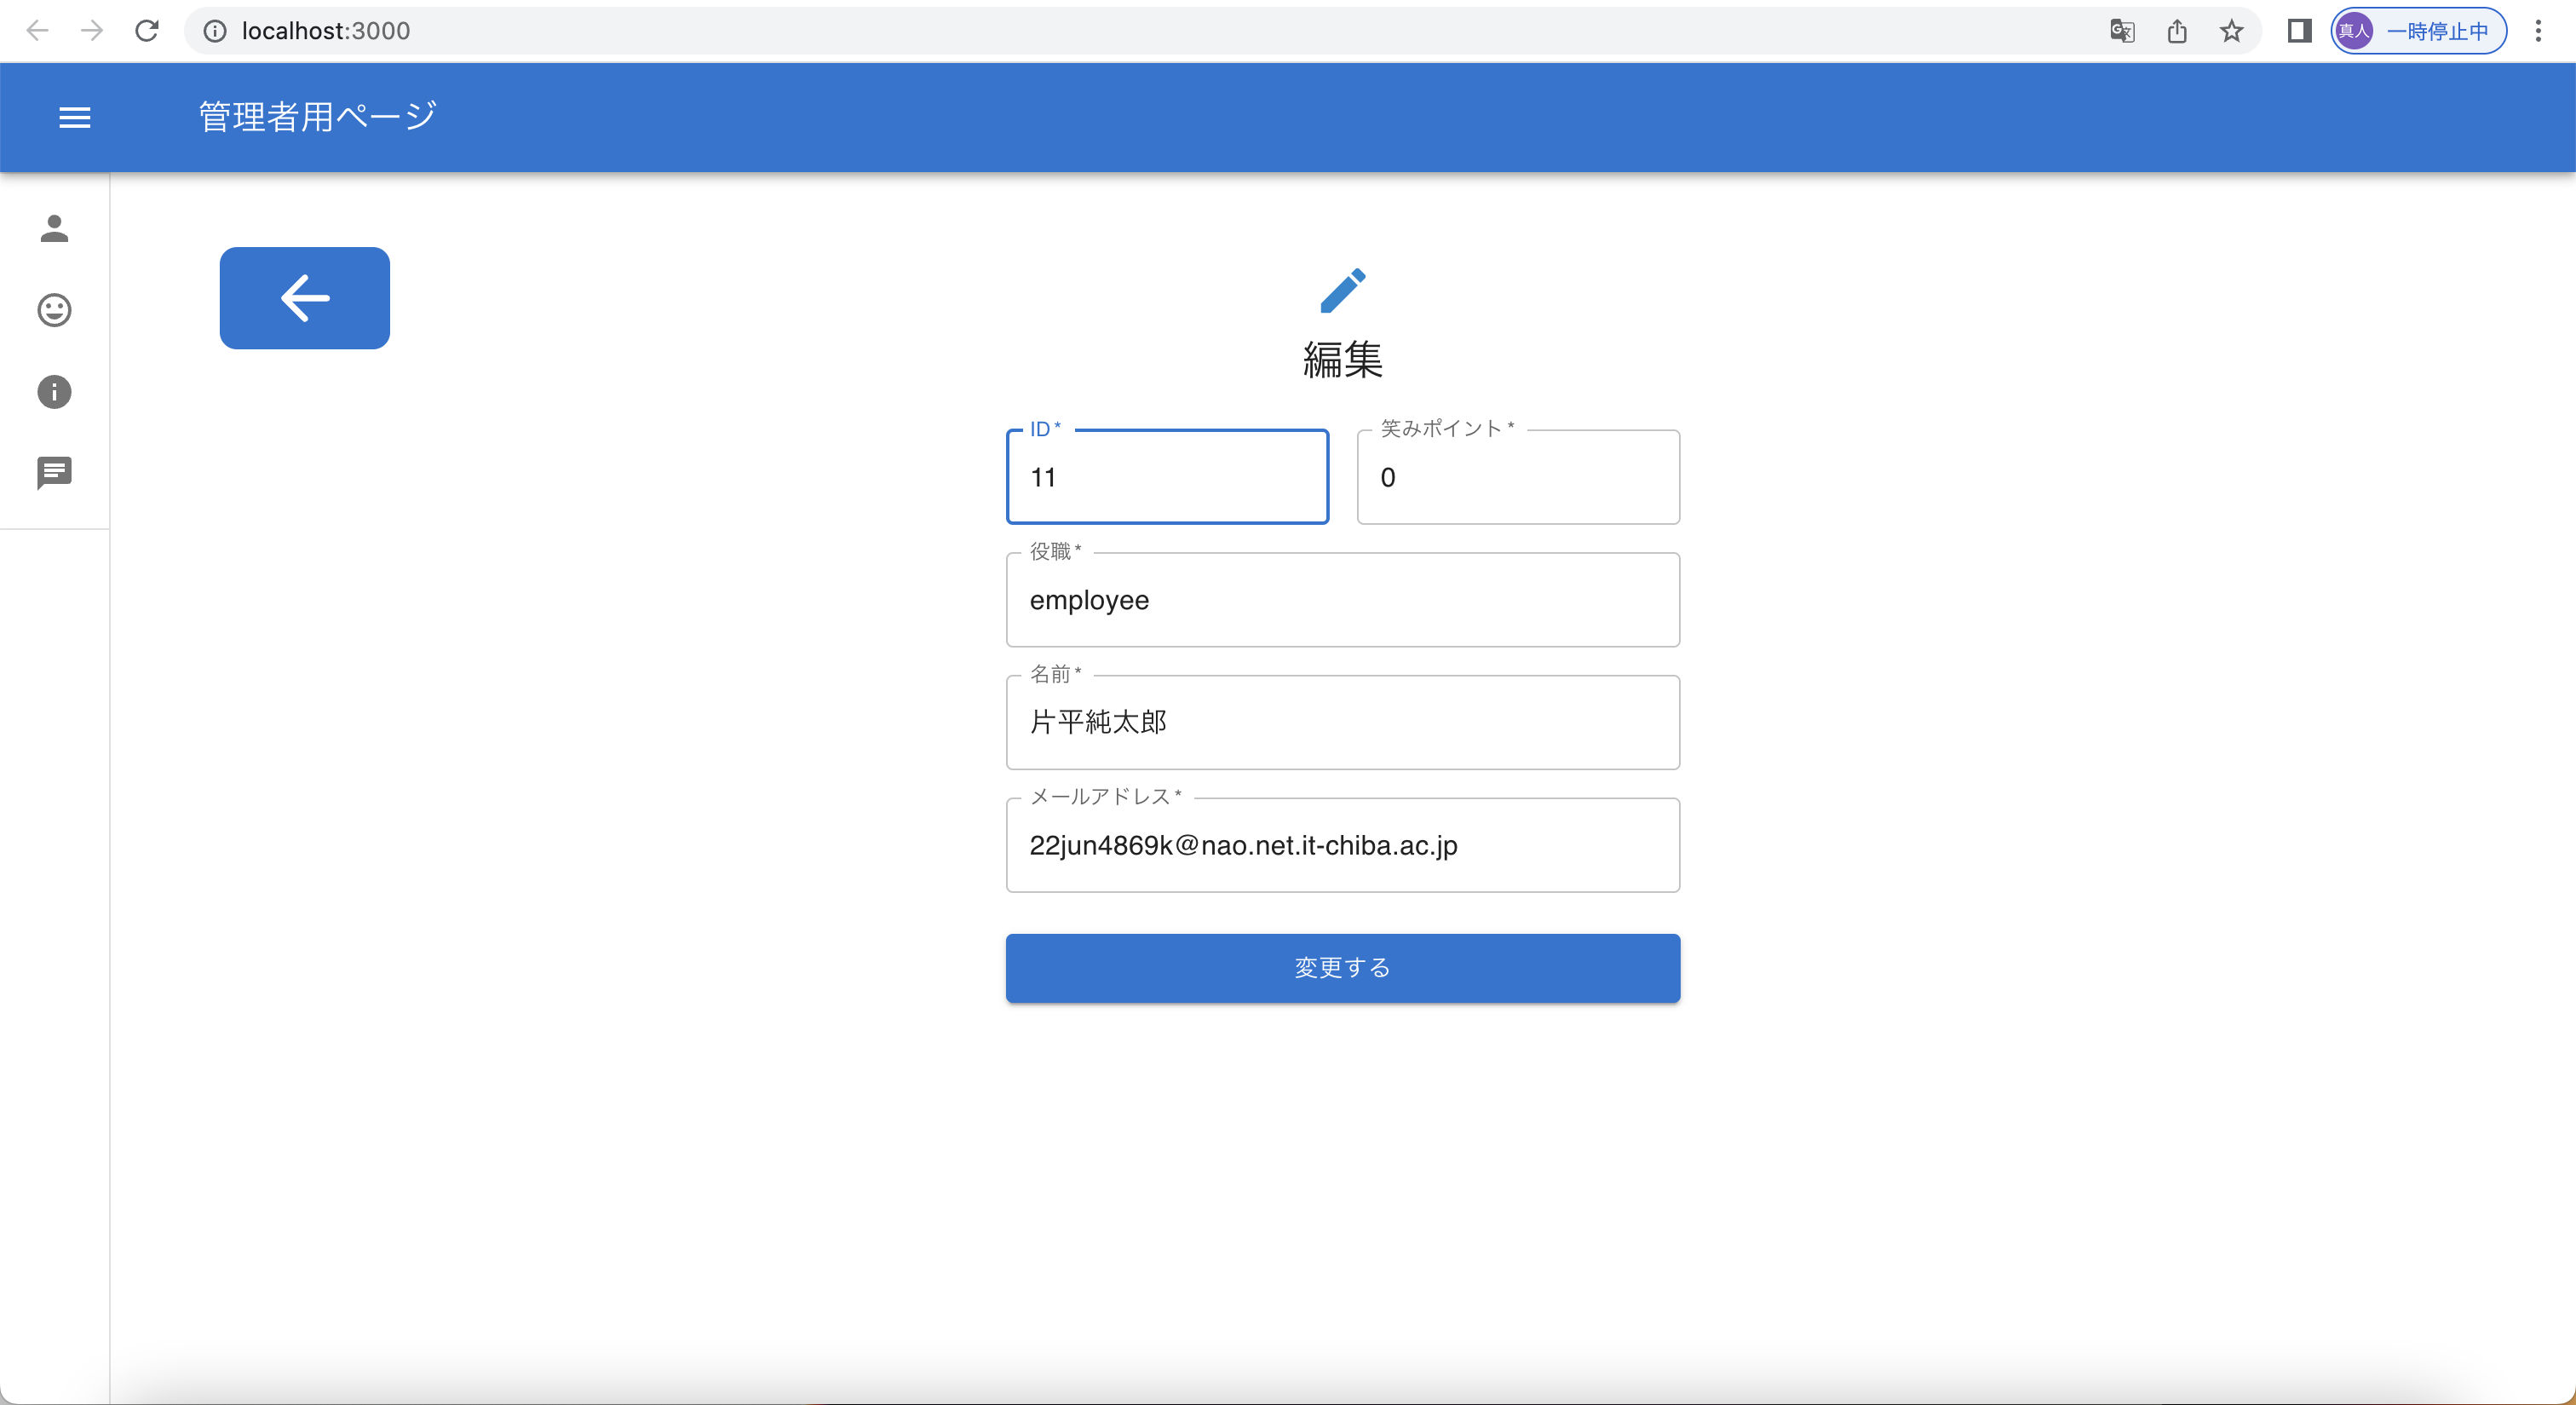
\includegraphics[scale=0.3, clip]{./img/sample7.png}
			\caption{編集画面}
			\label{fig:図の名前}
	\end{center}
\end{figure}

\clearpage

\begin{figure}[!h]
	\begin{center}
			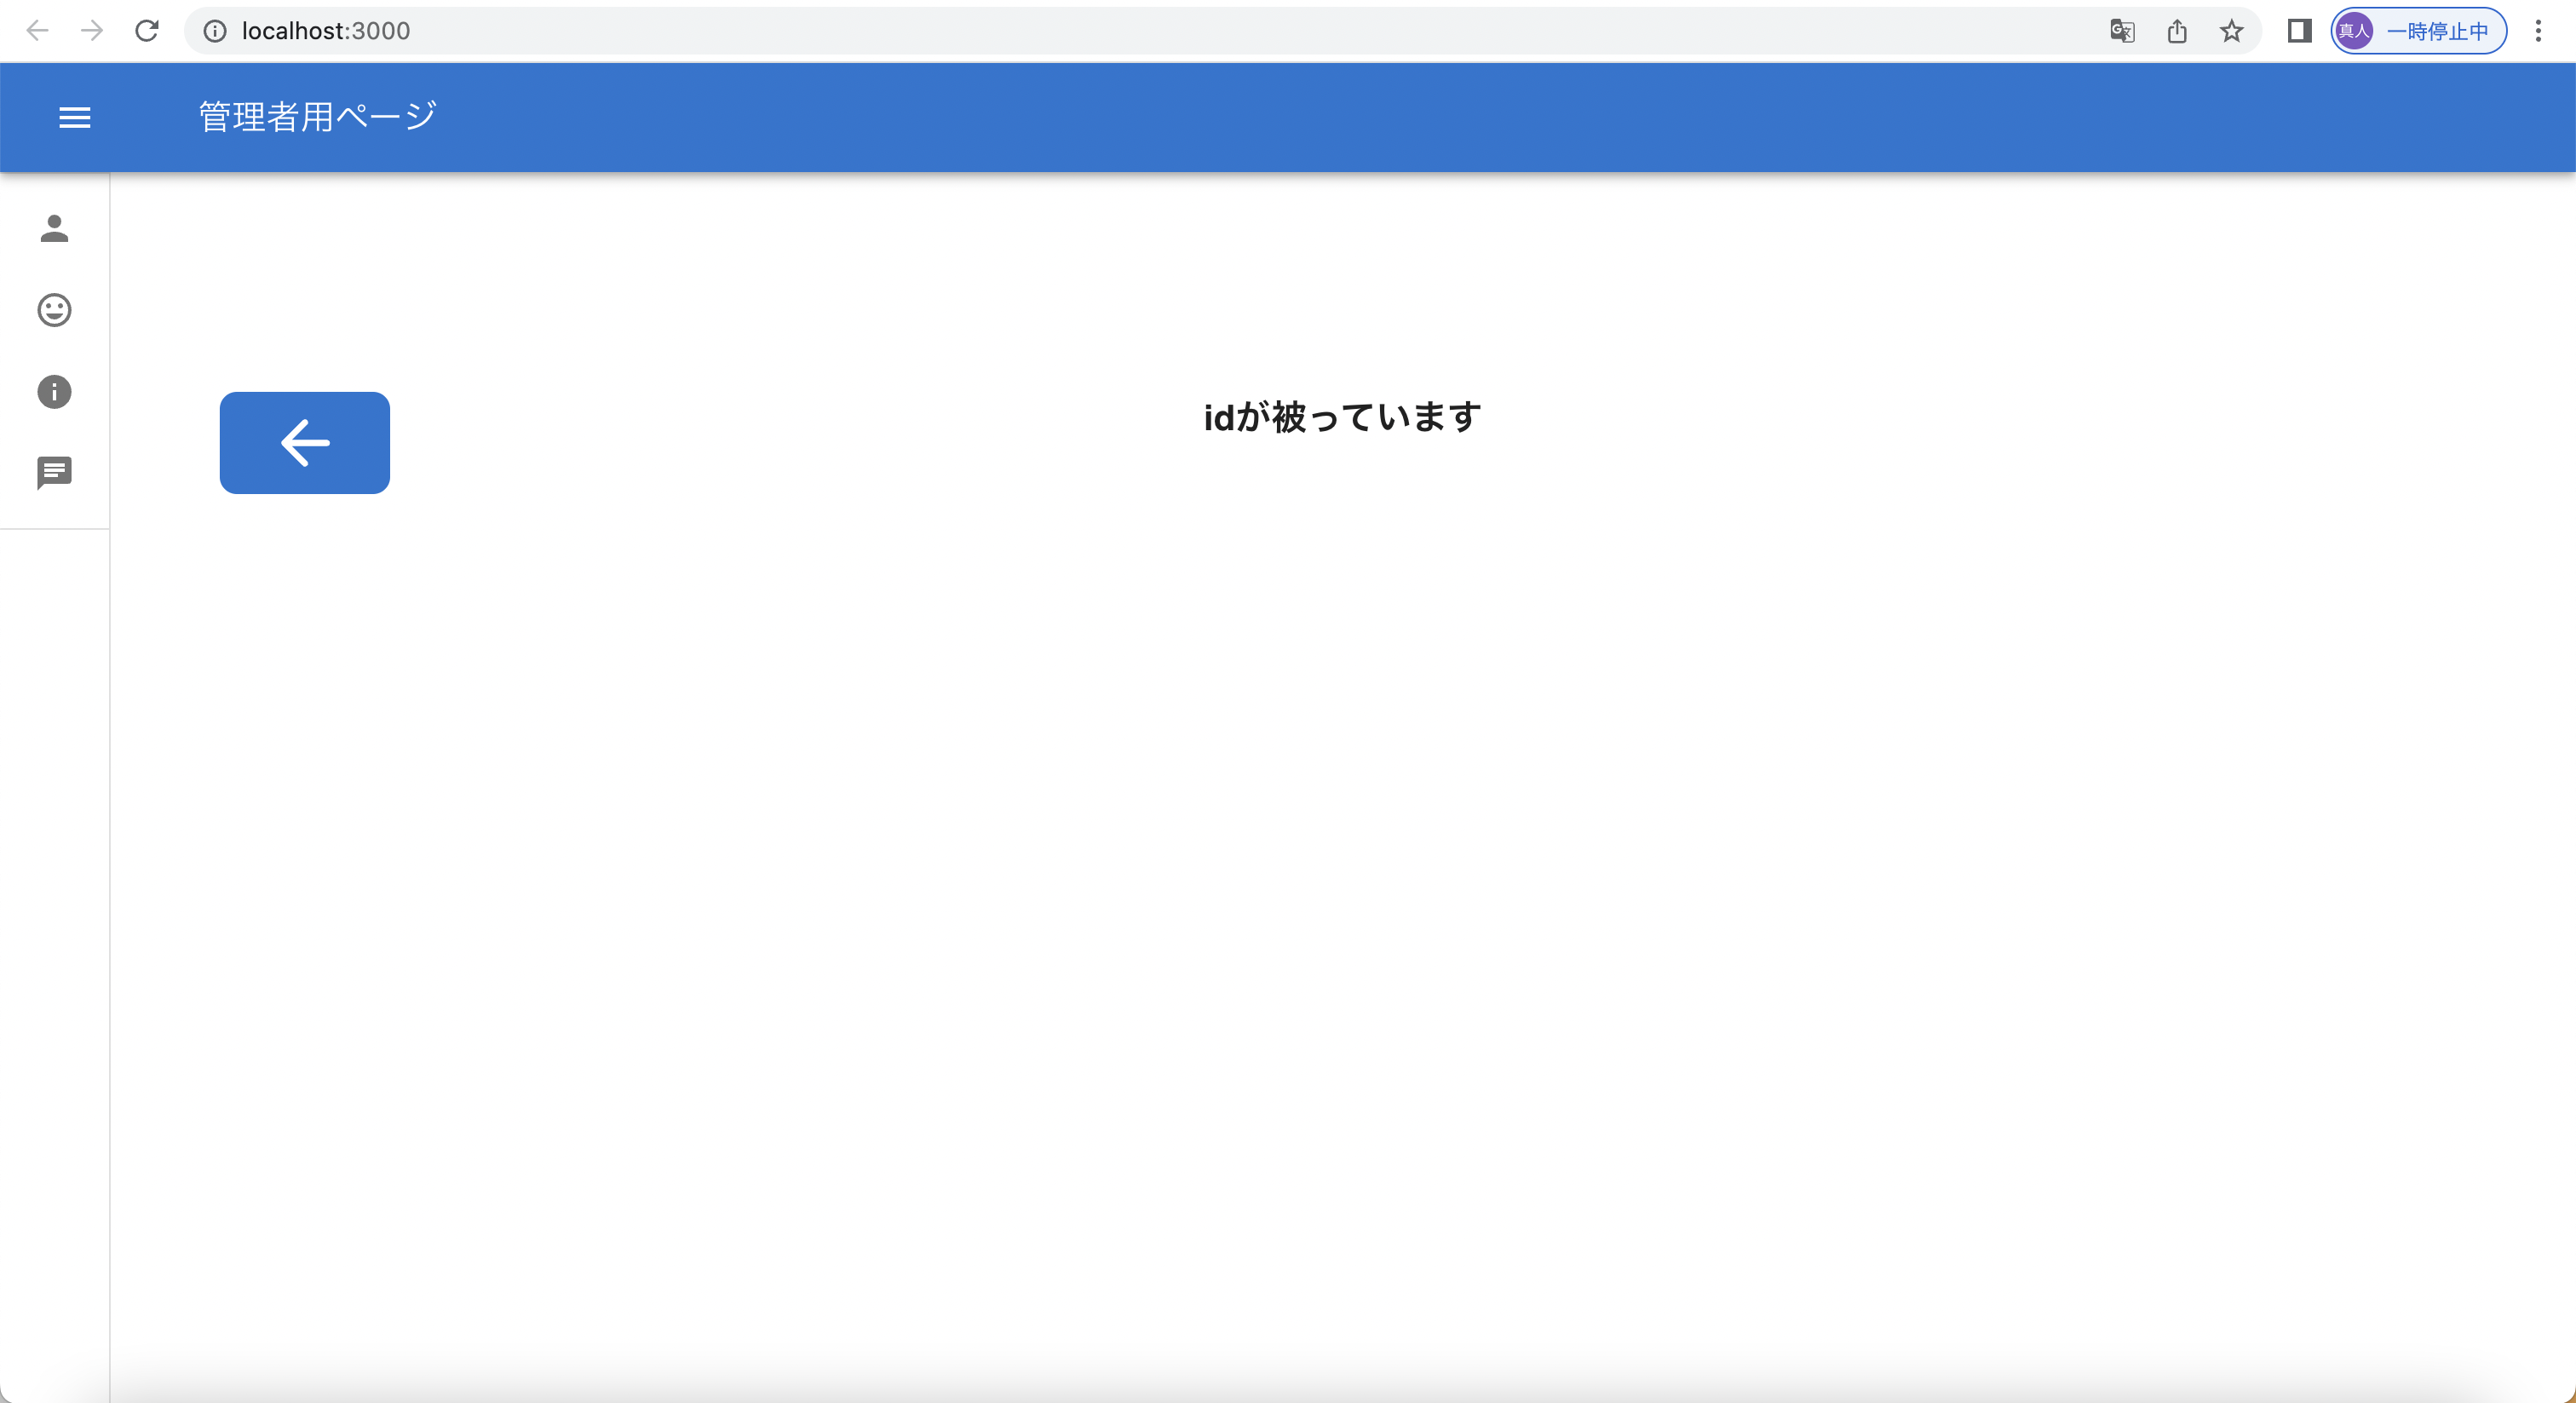
\includegraphics[scale=0.3, clip]{./img/sample8.png}
			\caption{idが被っている際の画面}
			\label{fig:図の名前}
	\end{center}
\end{figure}

\subsection{社員の顔写真閲覧機能}
社員の顔写真を閲覧できるページは図4.6の社員管理画面の詳細ボタンから移動できる.
移動すると過去5日分の写真の笑顔度の傾向に関してのグラフを表示している.
図4.9にそのスクリーンショットを示す.
提出されている写真が一枚も無い,または一枚のみの場合は笑顔度の傾向に関してのグラフを
表示しない様にした(図4.10).
日付のボタンは今日から4日前までの5日分あり,押すとそれぞれの日付で提出された社員の顔写真と
その顔を表情分析したグラフが表示される(図4.11).
もしボタンを押した日付の顔写真が提出されていなかったら図4.12の様になる.

\begin{figure}[!h]
	\begin{center}
			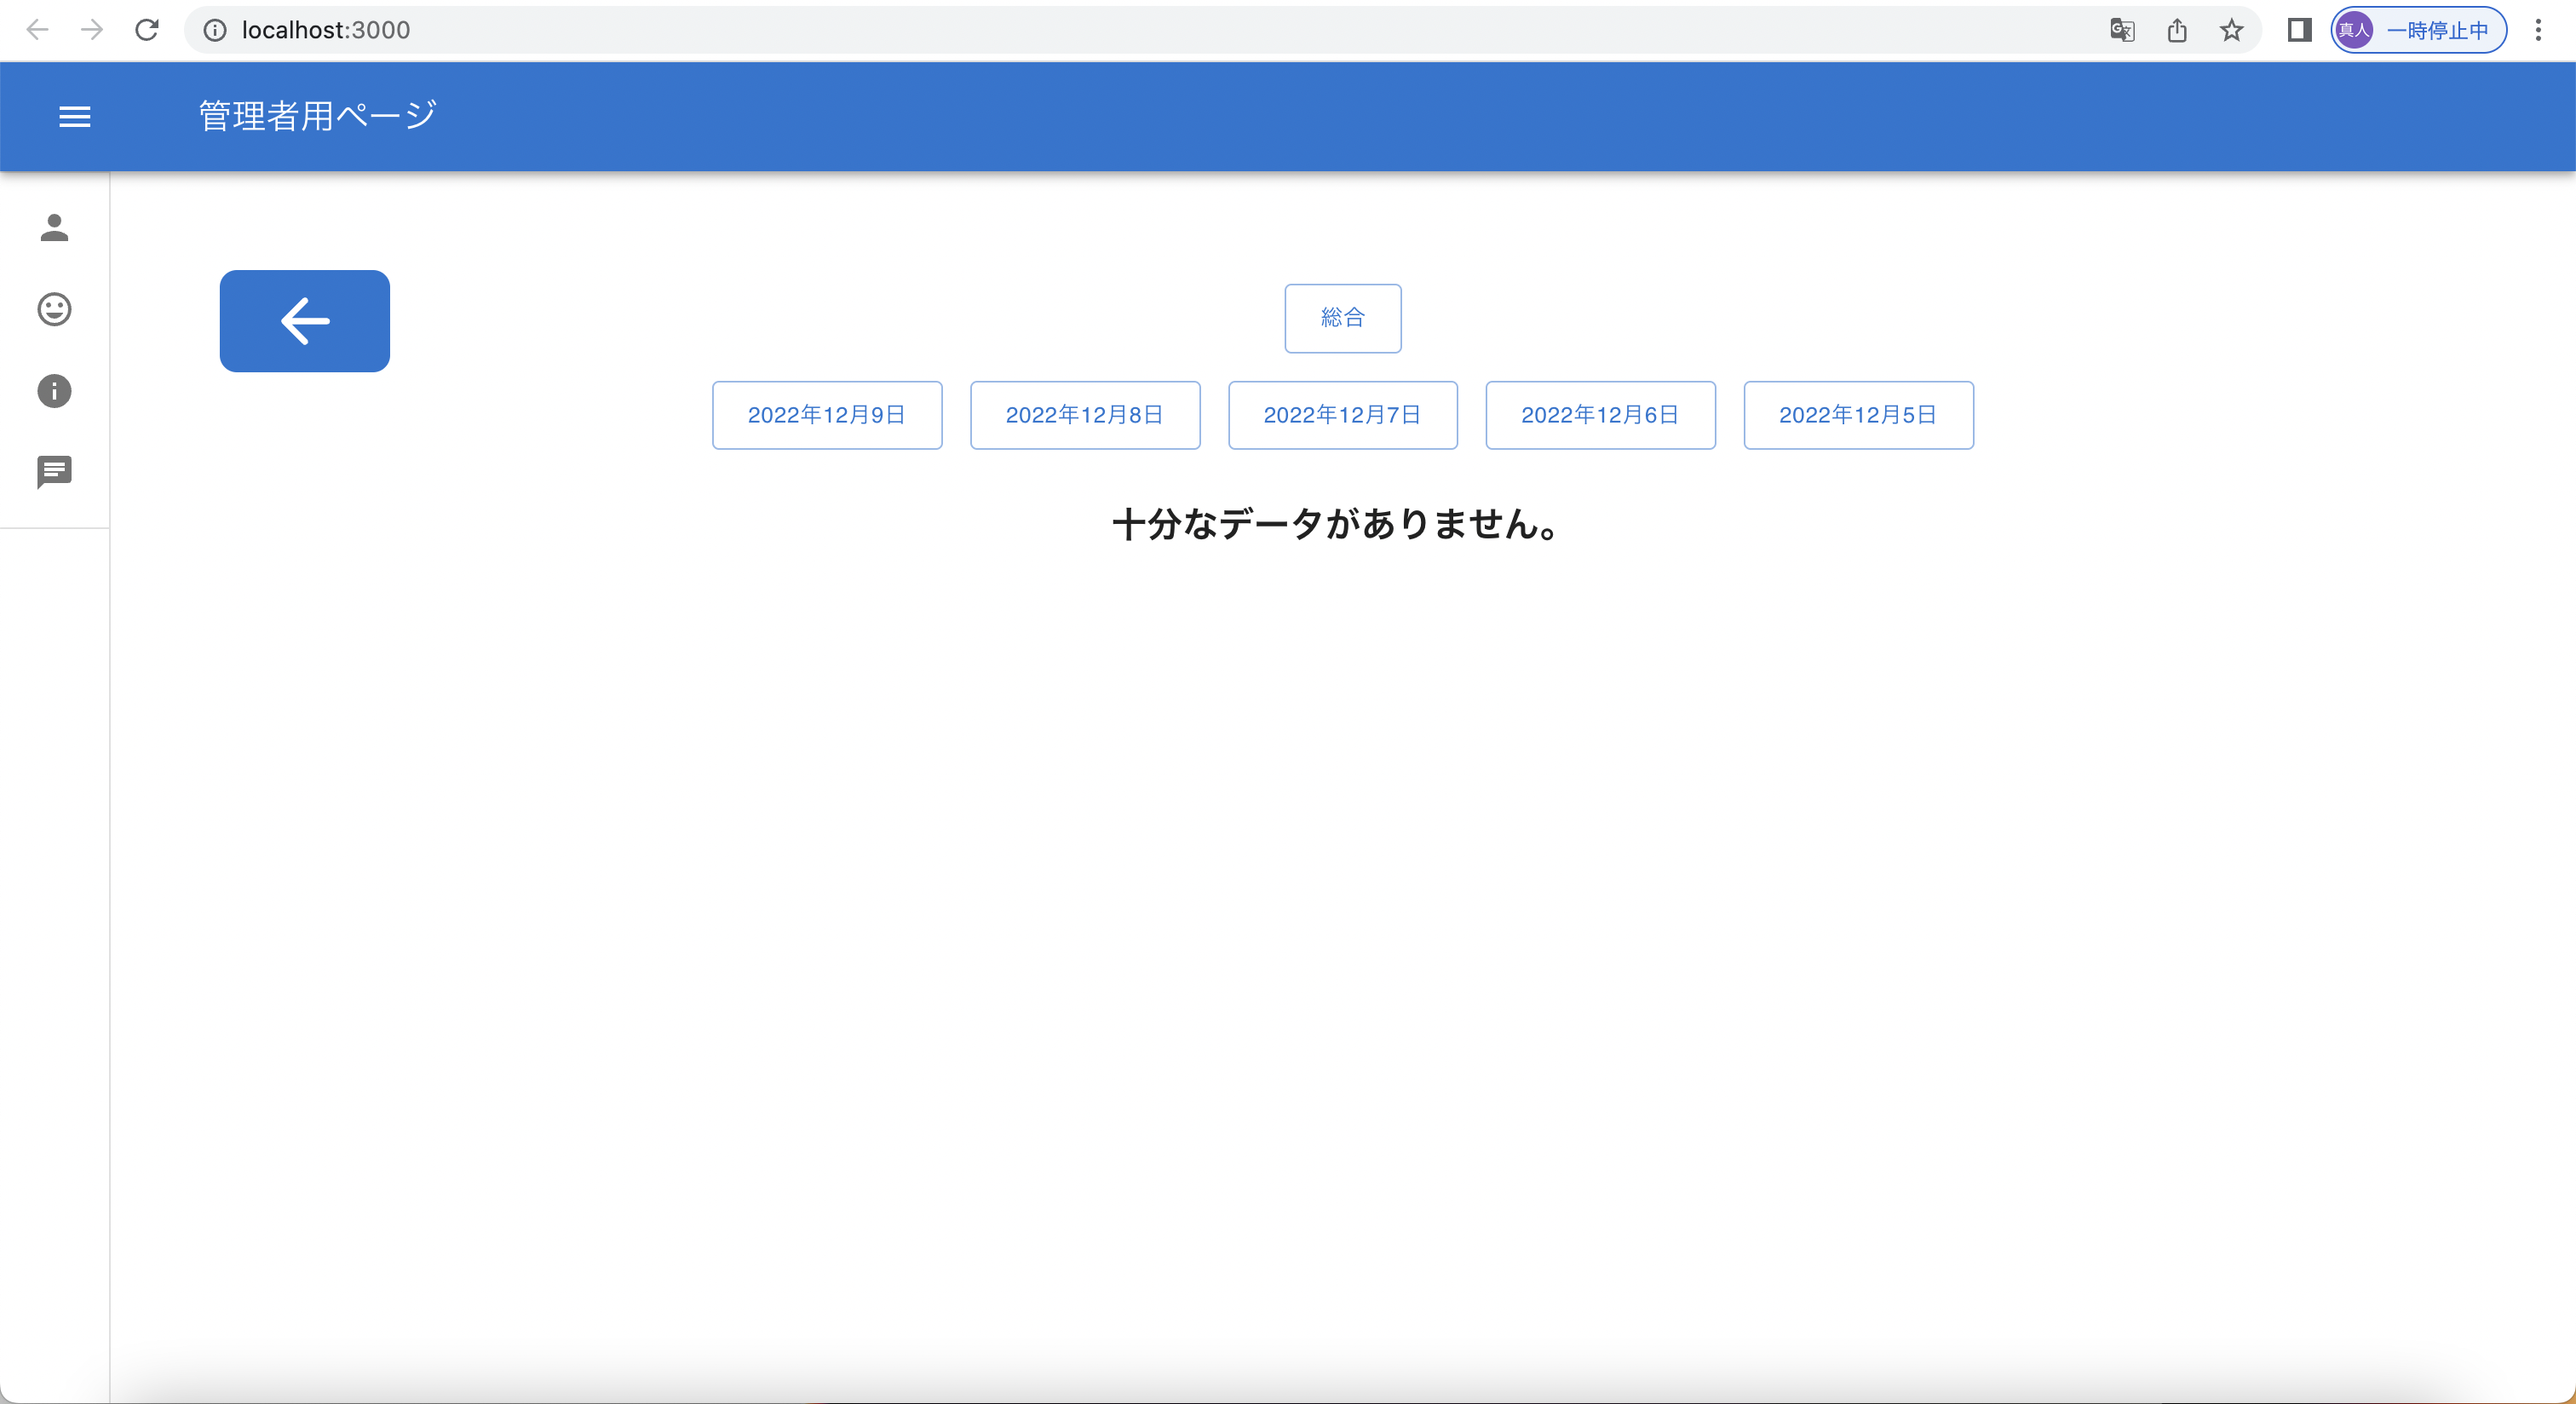
\includegraphics[scale=0.3, clip]{./img/sample9.png}
			\caption{顔写真閲覧画面}
			\label{fig:図の名前}
	\end{center}
\end{figure}

\begin{figure}[!h]
	\begin{center}
			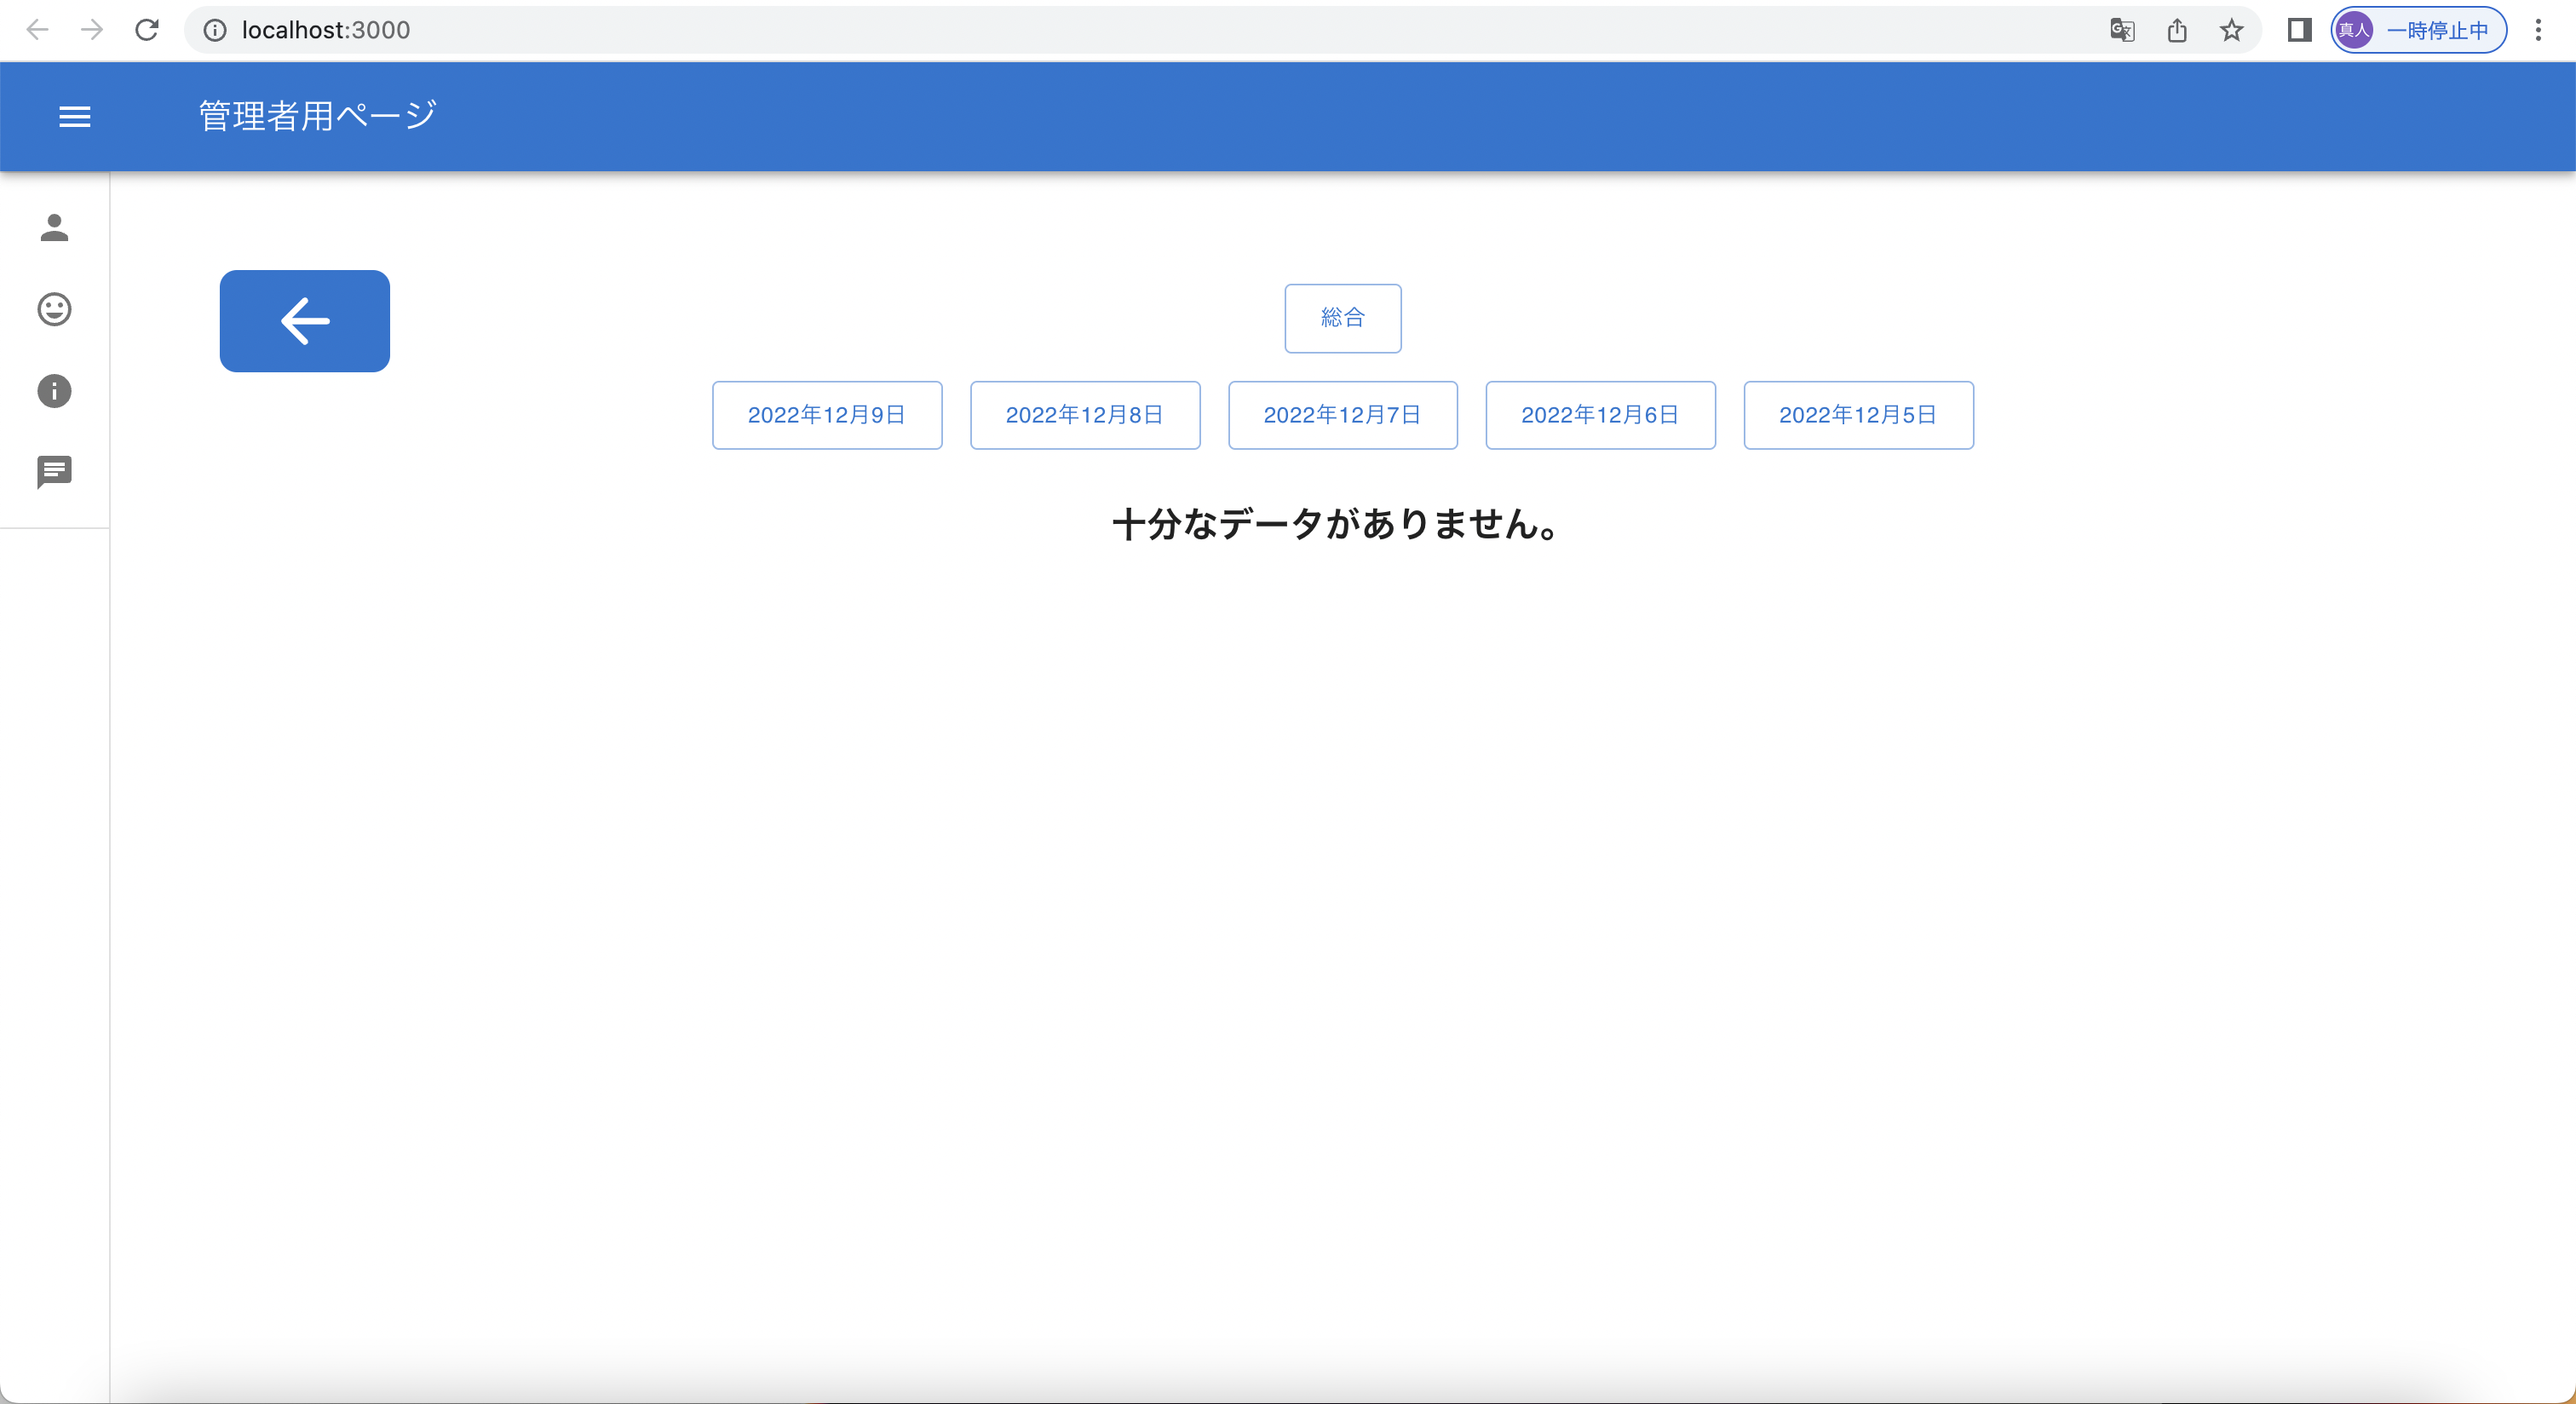
\includegraphics[scale=0.3, clip]{./img/sample9.png}
			\caption{笑顔度傾向グラフ非表示画面}
			\label{fig:図の名前}
	\end{center}
\end{figure}

\clearpage

\begin{figure}[!h]
	\begin{center}
			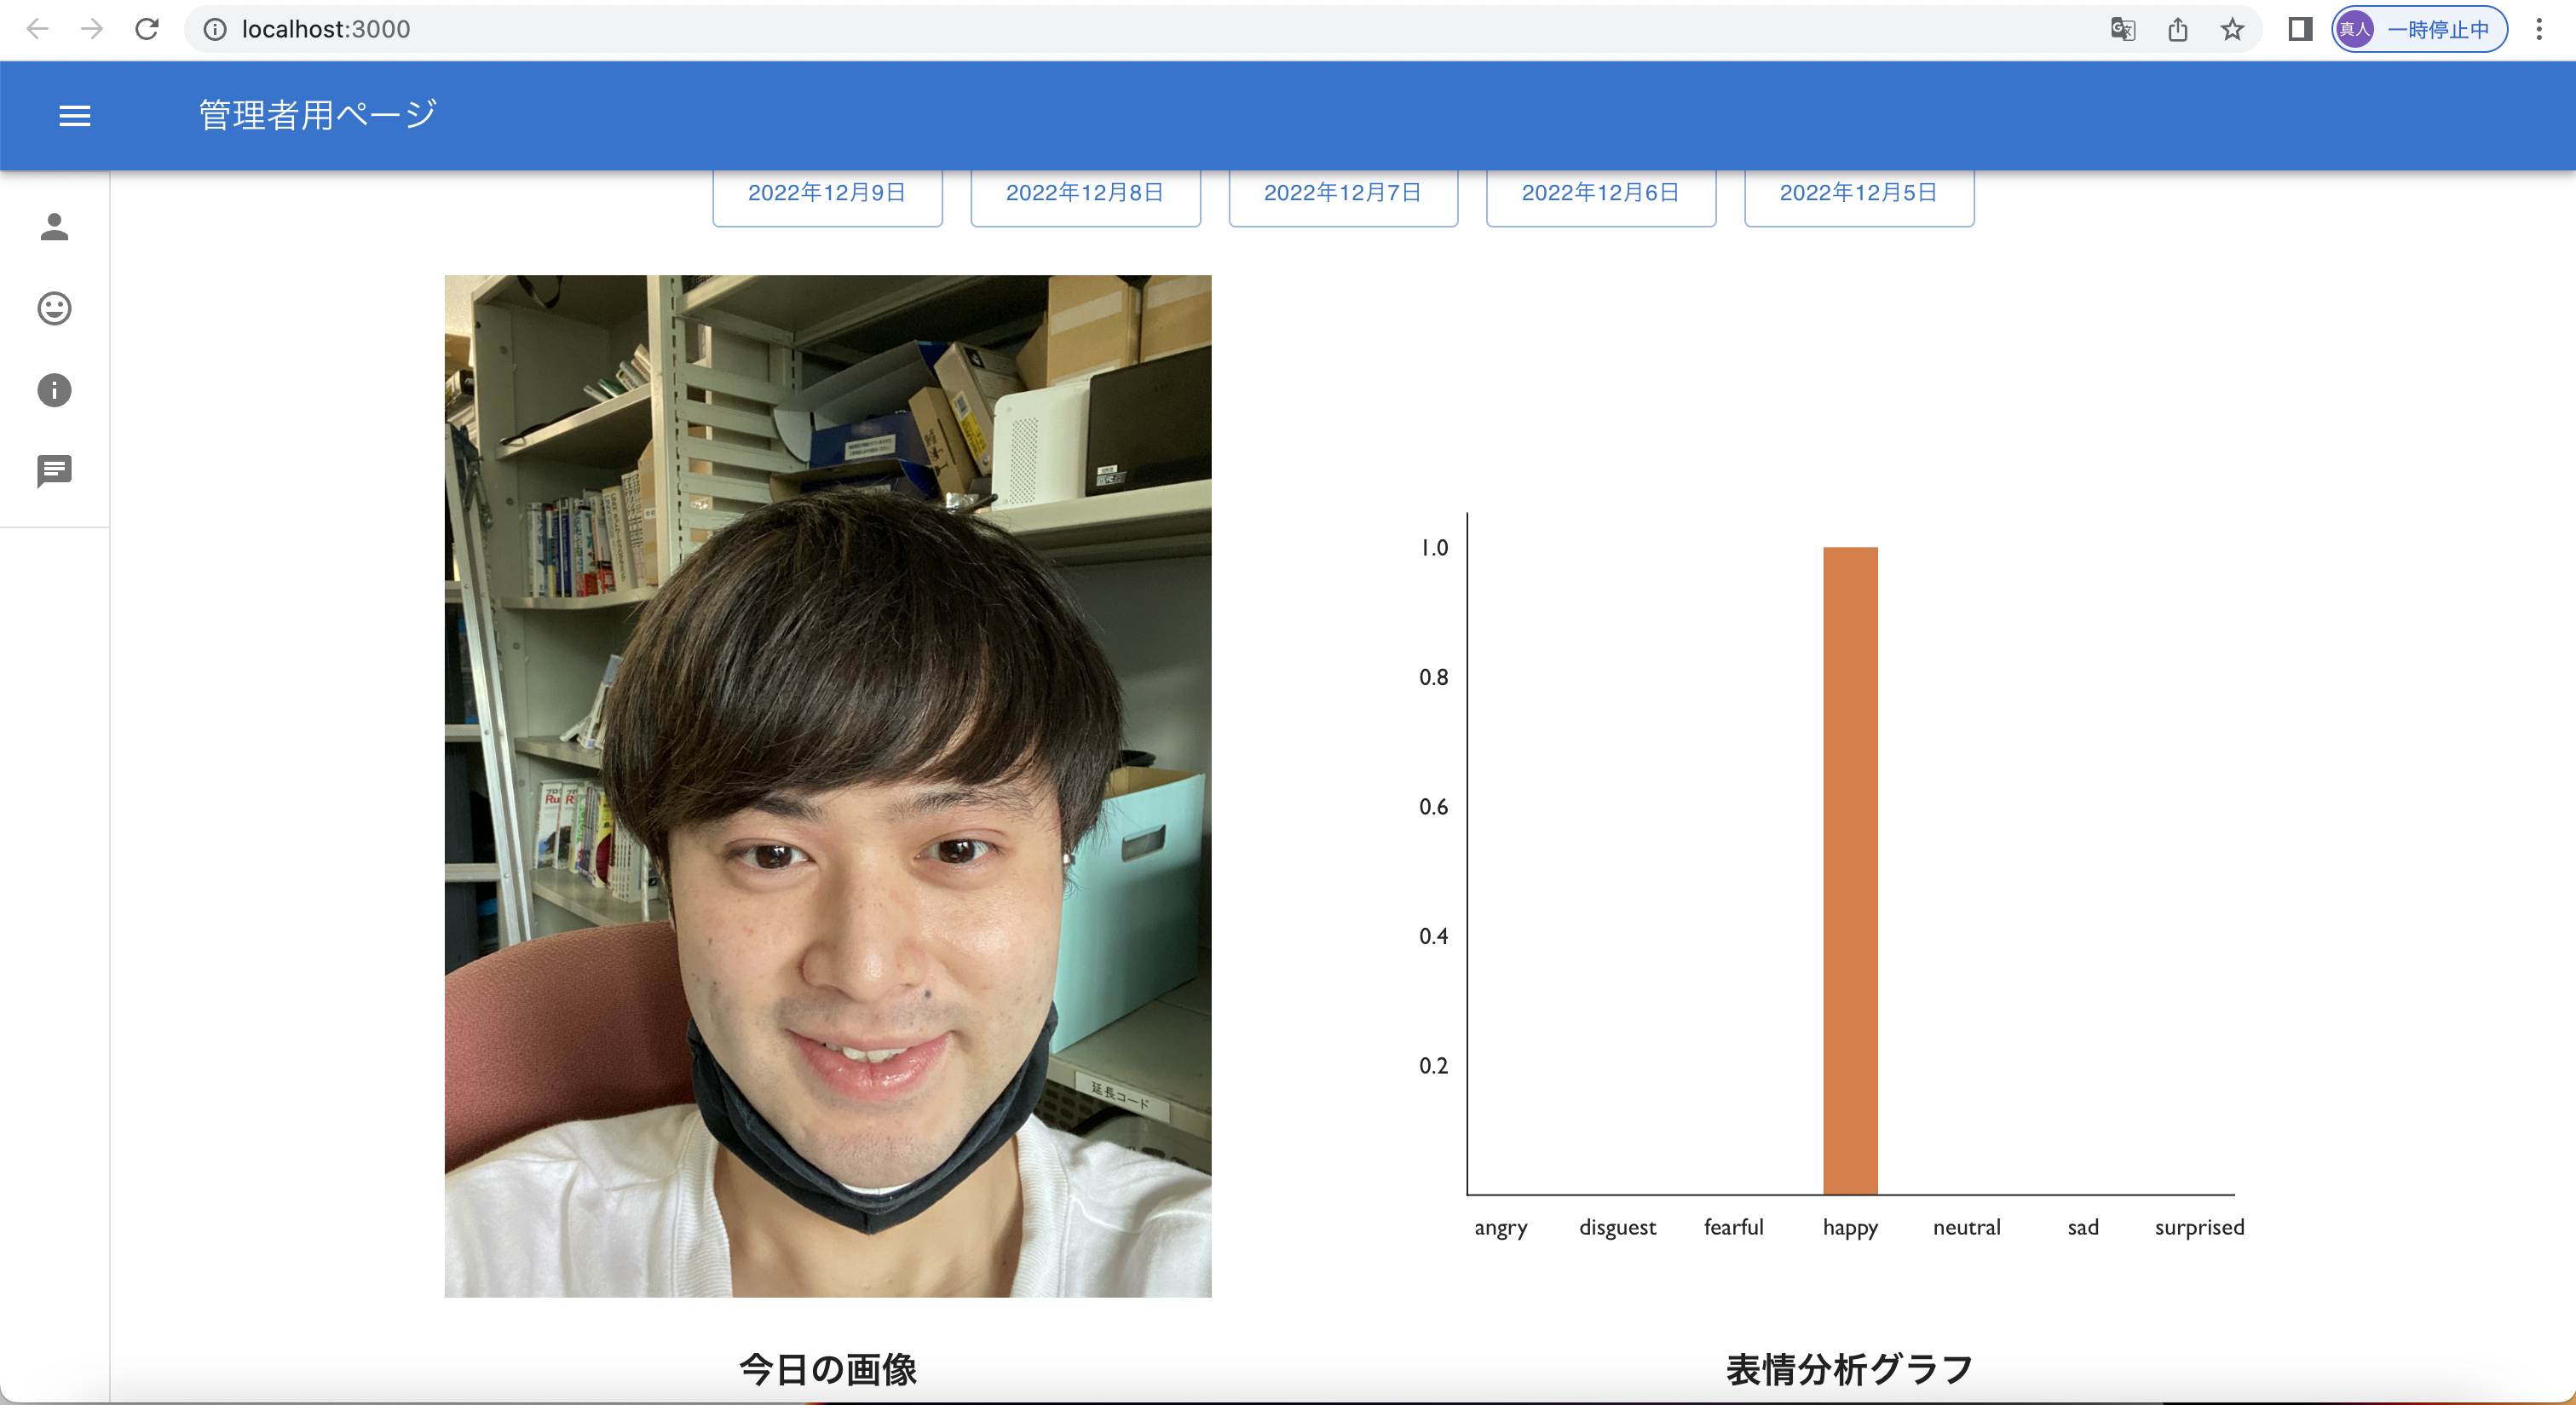
\includegraphics[scale=0.3, clip]{./img/sample10.png}
			\caption{日付のボタンを押した際の画面}
			\label{fig:図の名前}
	\end{center}
\end{figure}

\begin{figure}[!h]
	\begin{center}
			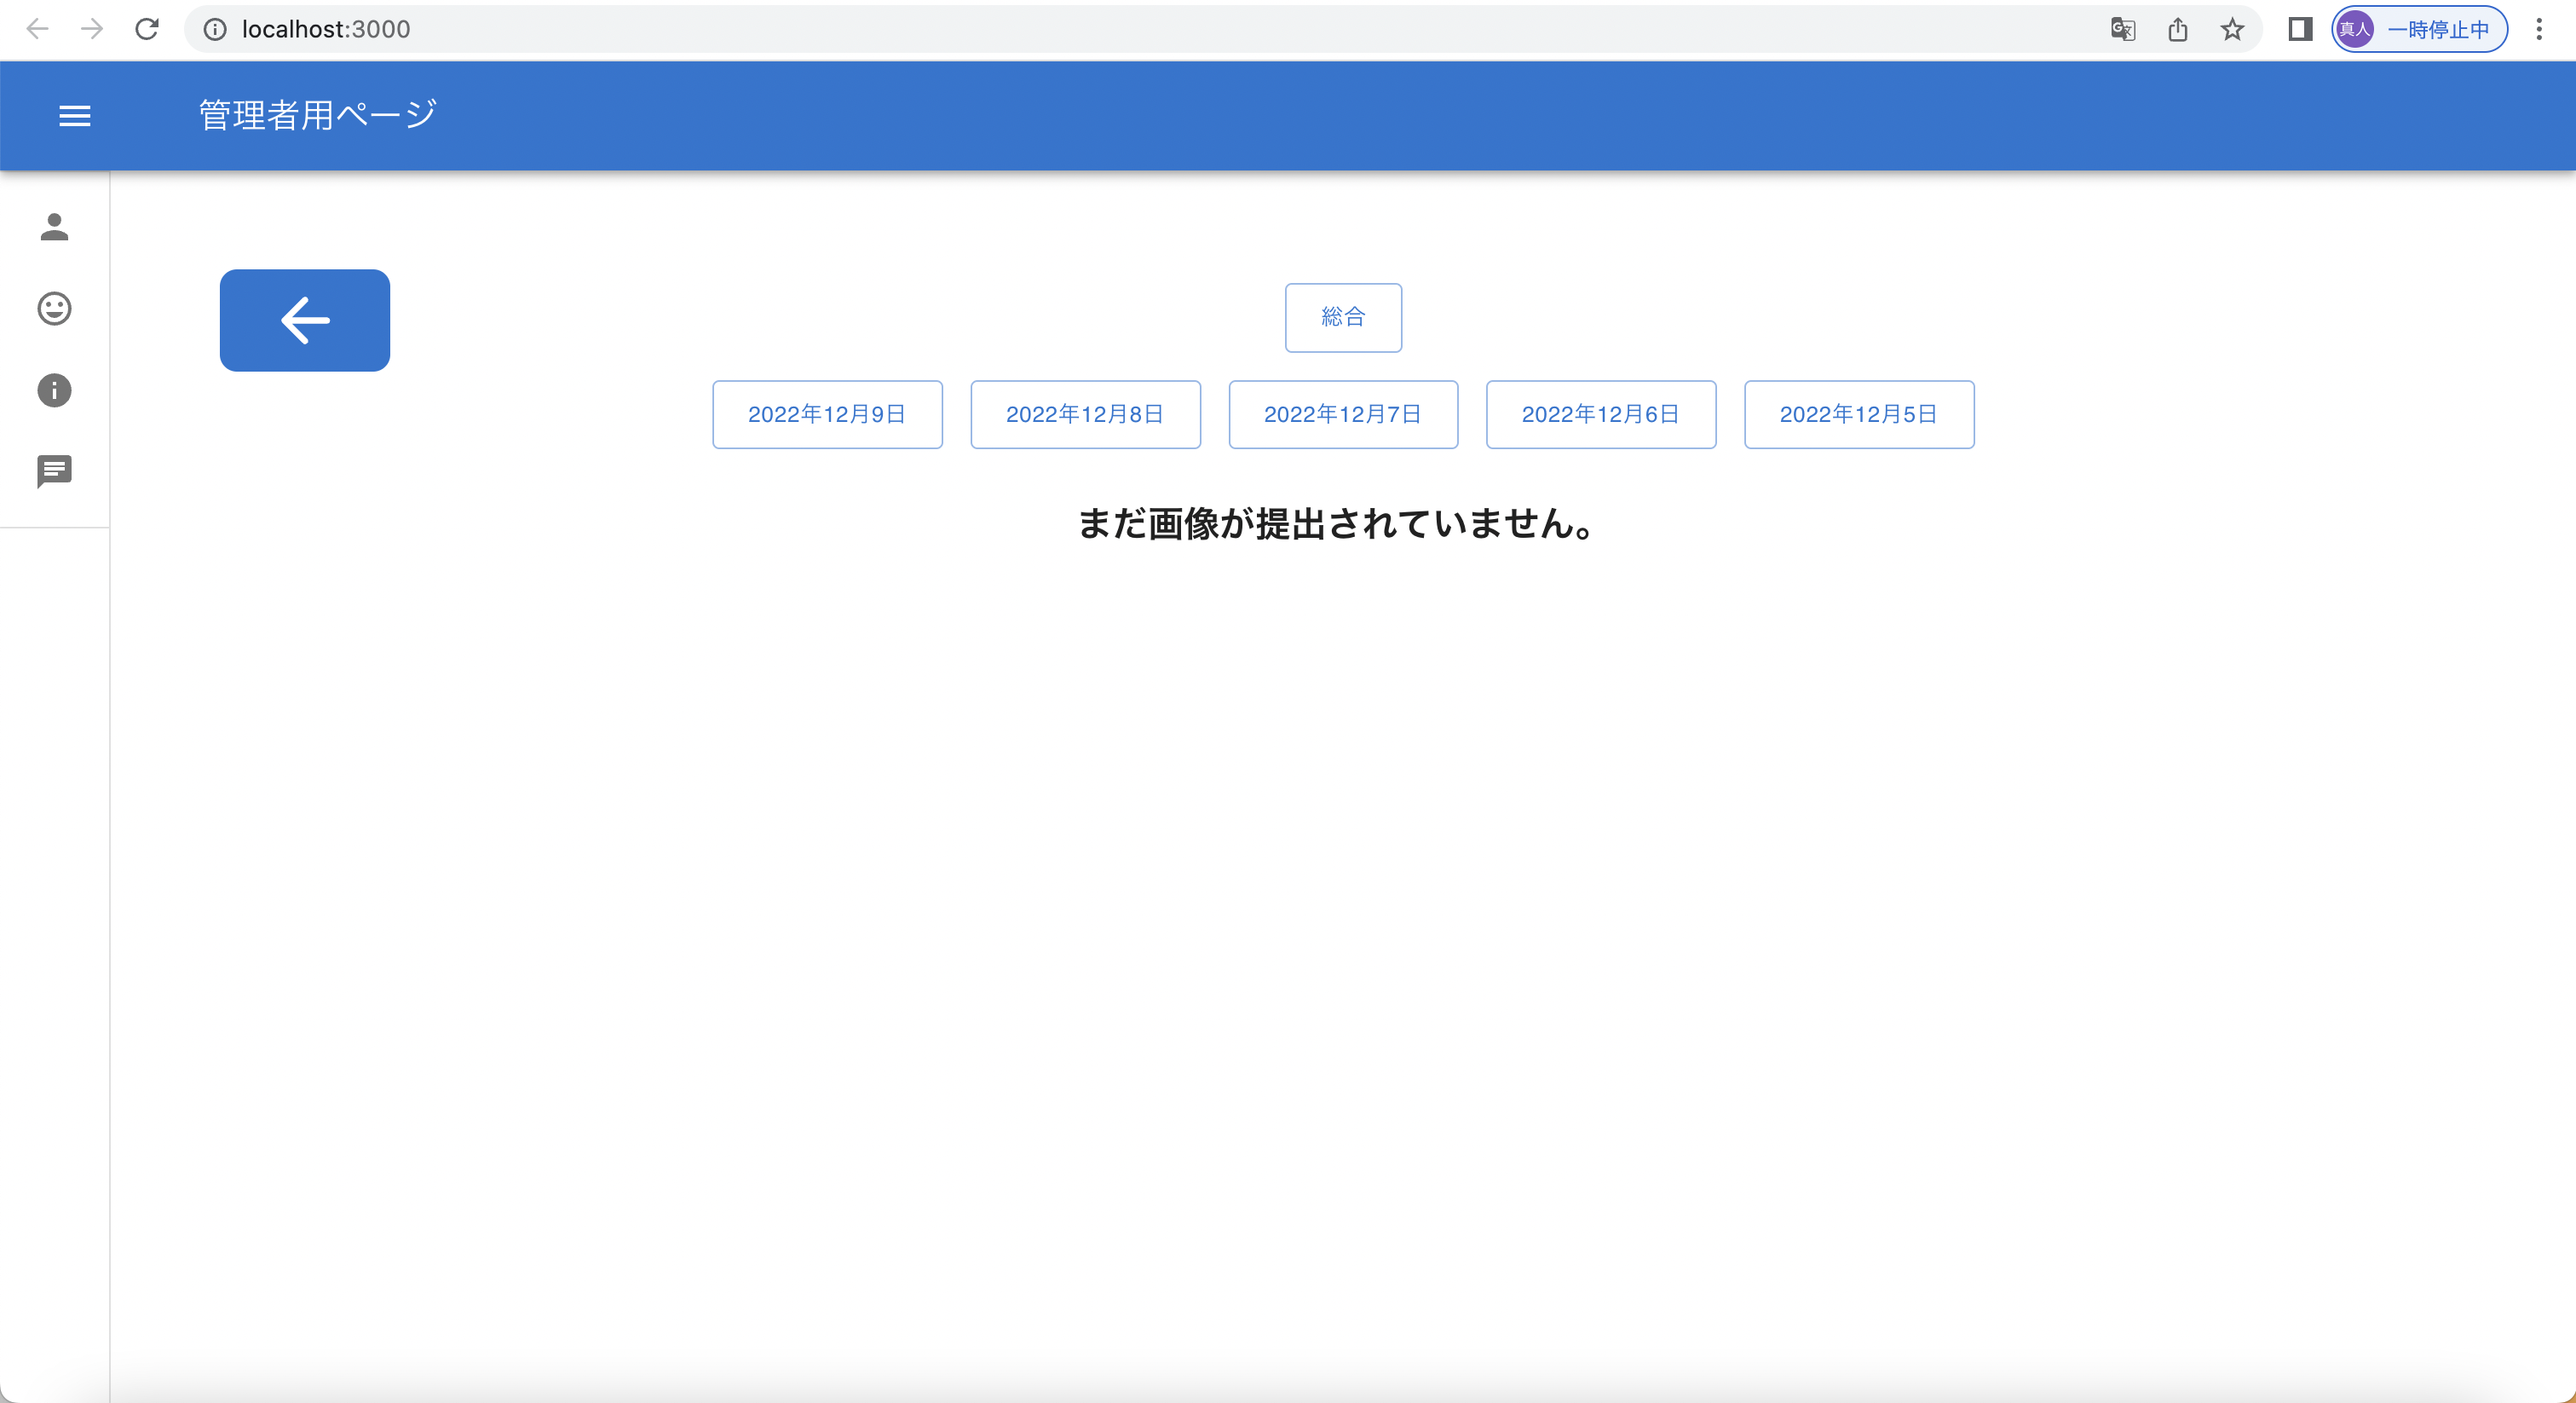
\includegraphics[scale=0.3, clip]{./img/sample11.png}
			\caption{写真が提出されていなかった際の画面}
			\label{fig:図の名前}
	\end{center}
\end{figure}

\clearpage

\section{認証機能}

認証機能はFirebase Authenticationを利用している.今回はユーザーにログインさせる
方法としてGoogleサインインを実装した.
これを利用することによって,アカウント作成といった作業の省略や安全性を提供できる.
ログイン画面のスクリーンショットを図4.13,図4.14に,図4.15にログイン完了画面を示す.
\\

\vspace{17mm}

\begin{figure}[!h]
\begin{center}
  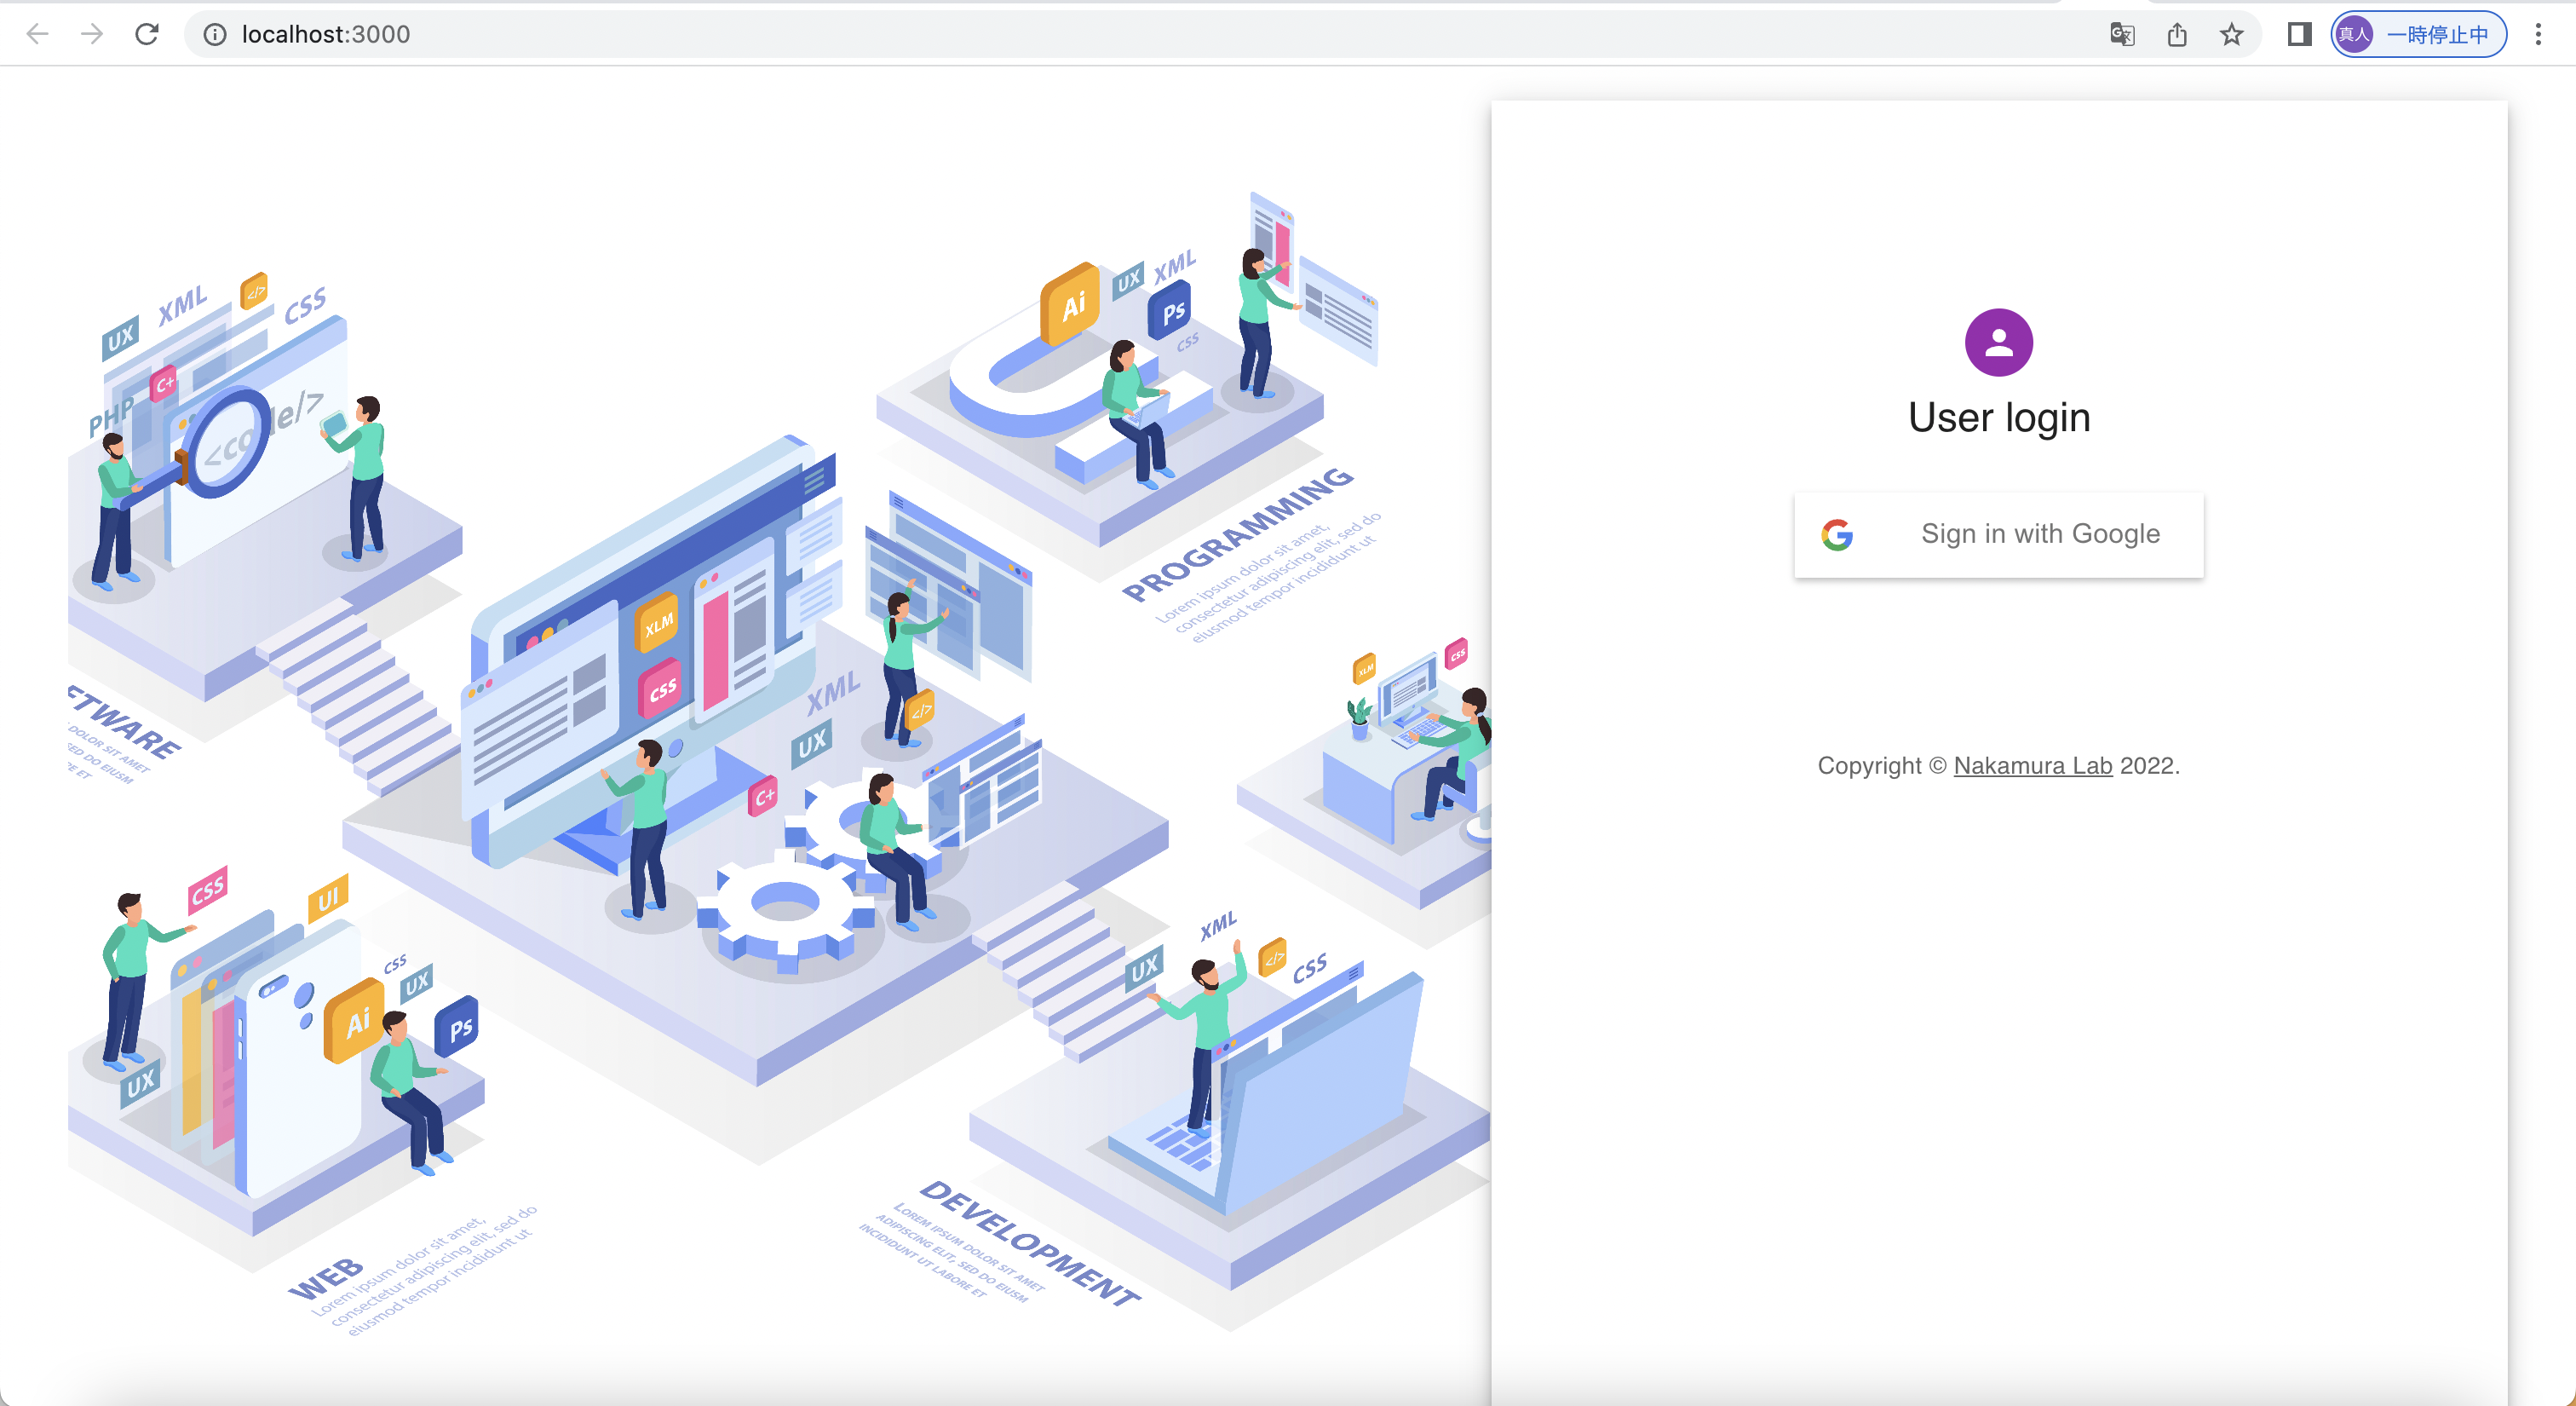
\includegraphics[scale=0.3, clip]{./img/sample13.png}
  \caption{ログイン画面}
  \label{fig:図の名前}
\end{center}
\end{figure}

\begin{figure}[!h]
  \begin{center}
    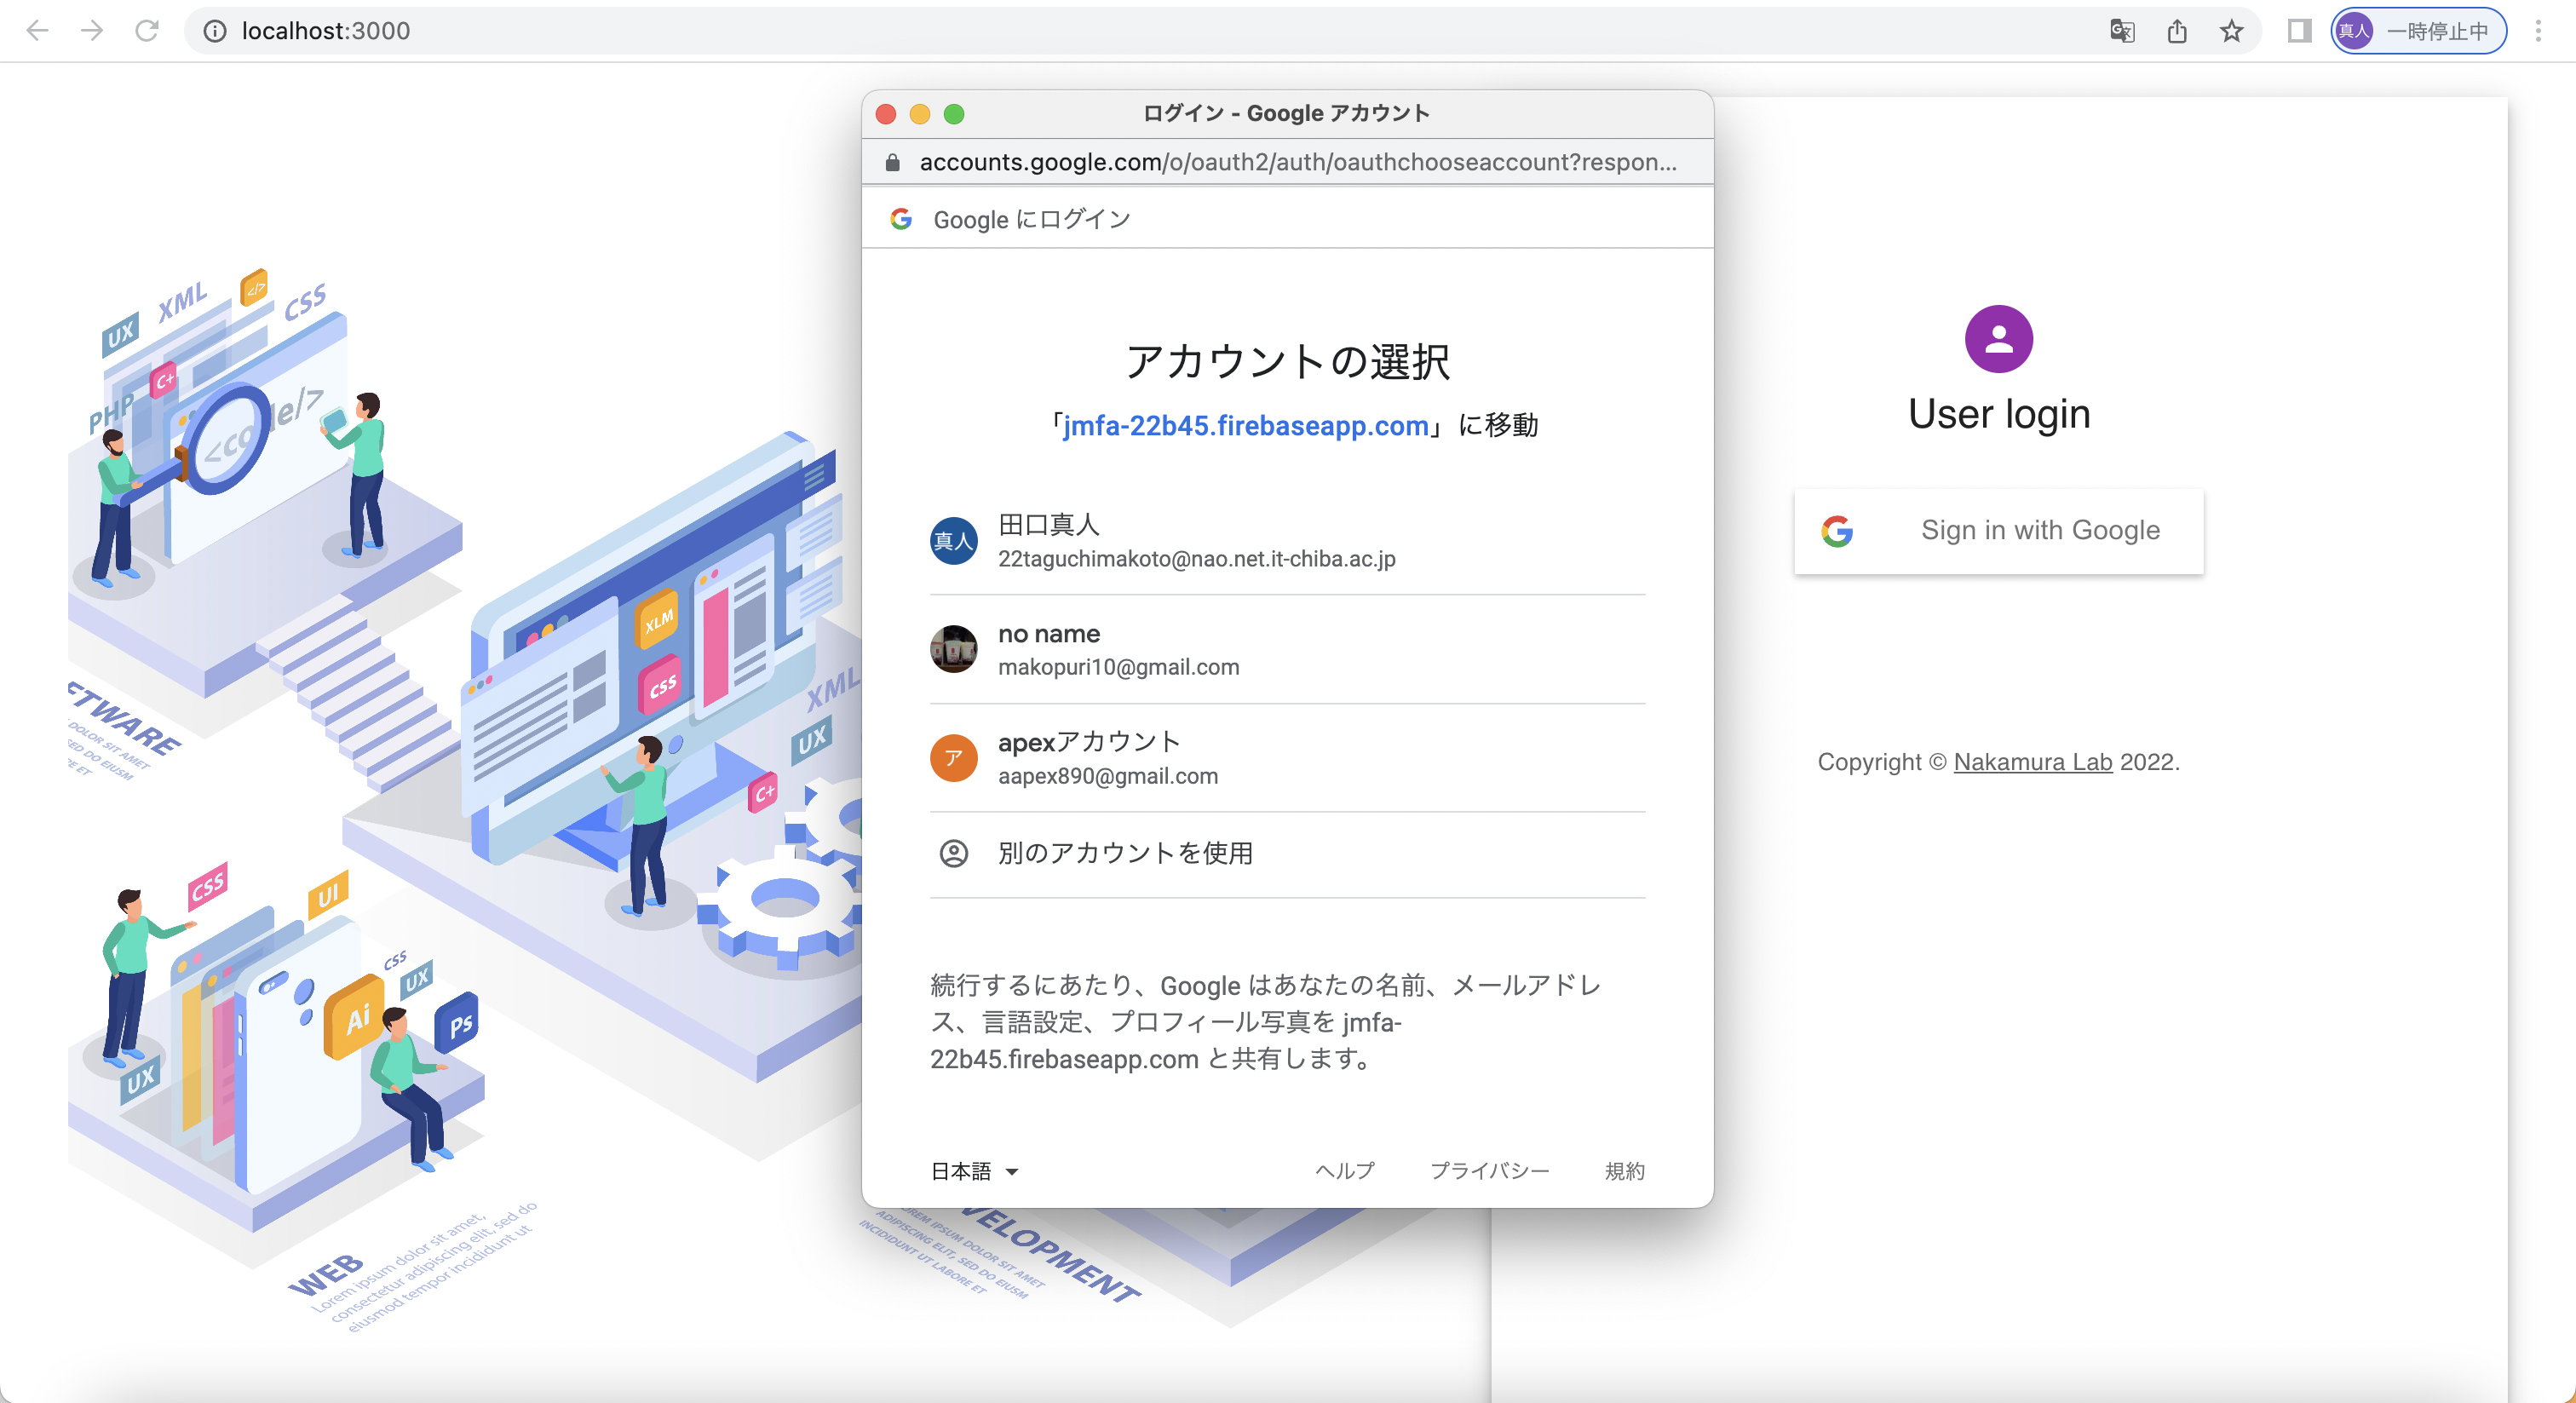
\includegraphics[scale=0.3, clip]{./img/sample14.png}
    \caption{アカウント選択画面}
    \label{fig:図の名前}
  \end{center}
  \end{figure}

  \begin{figure}[!h]
    \begin{center}
      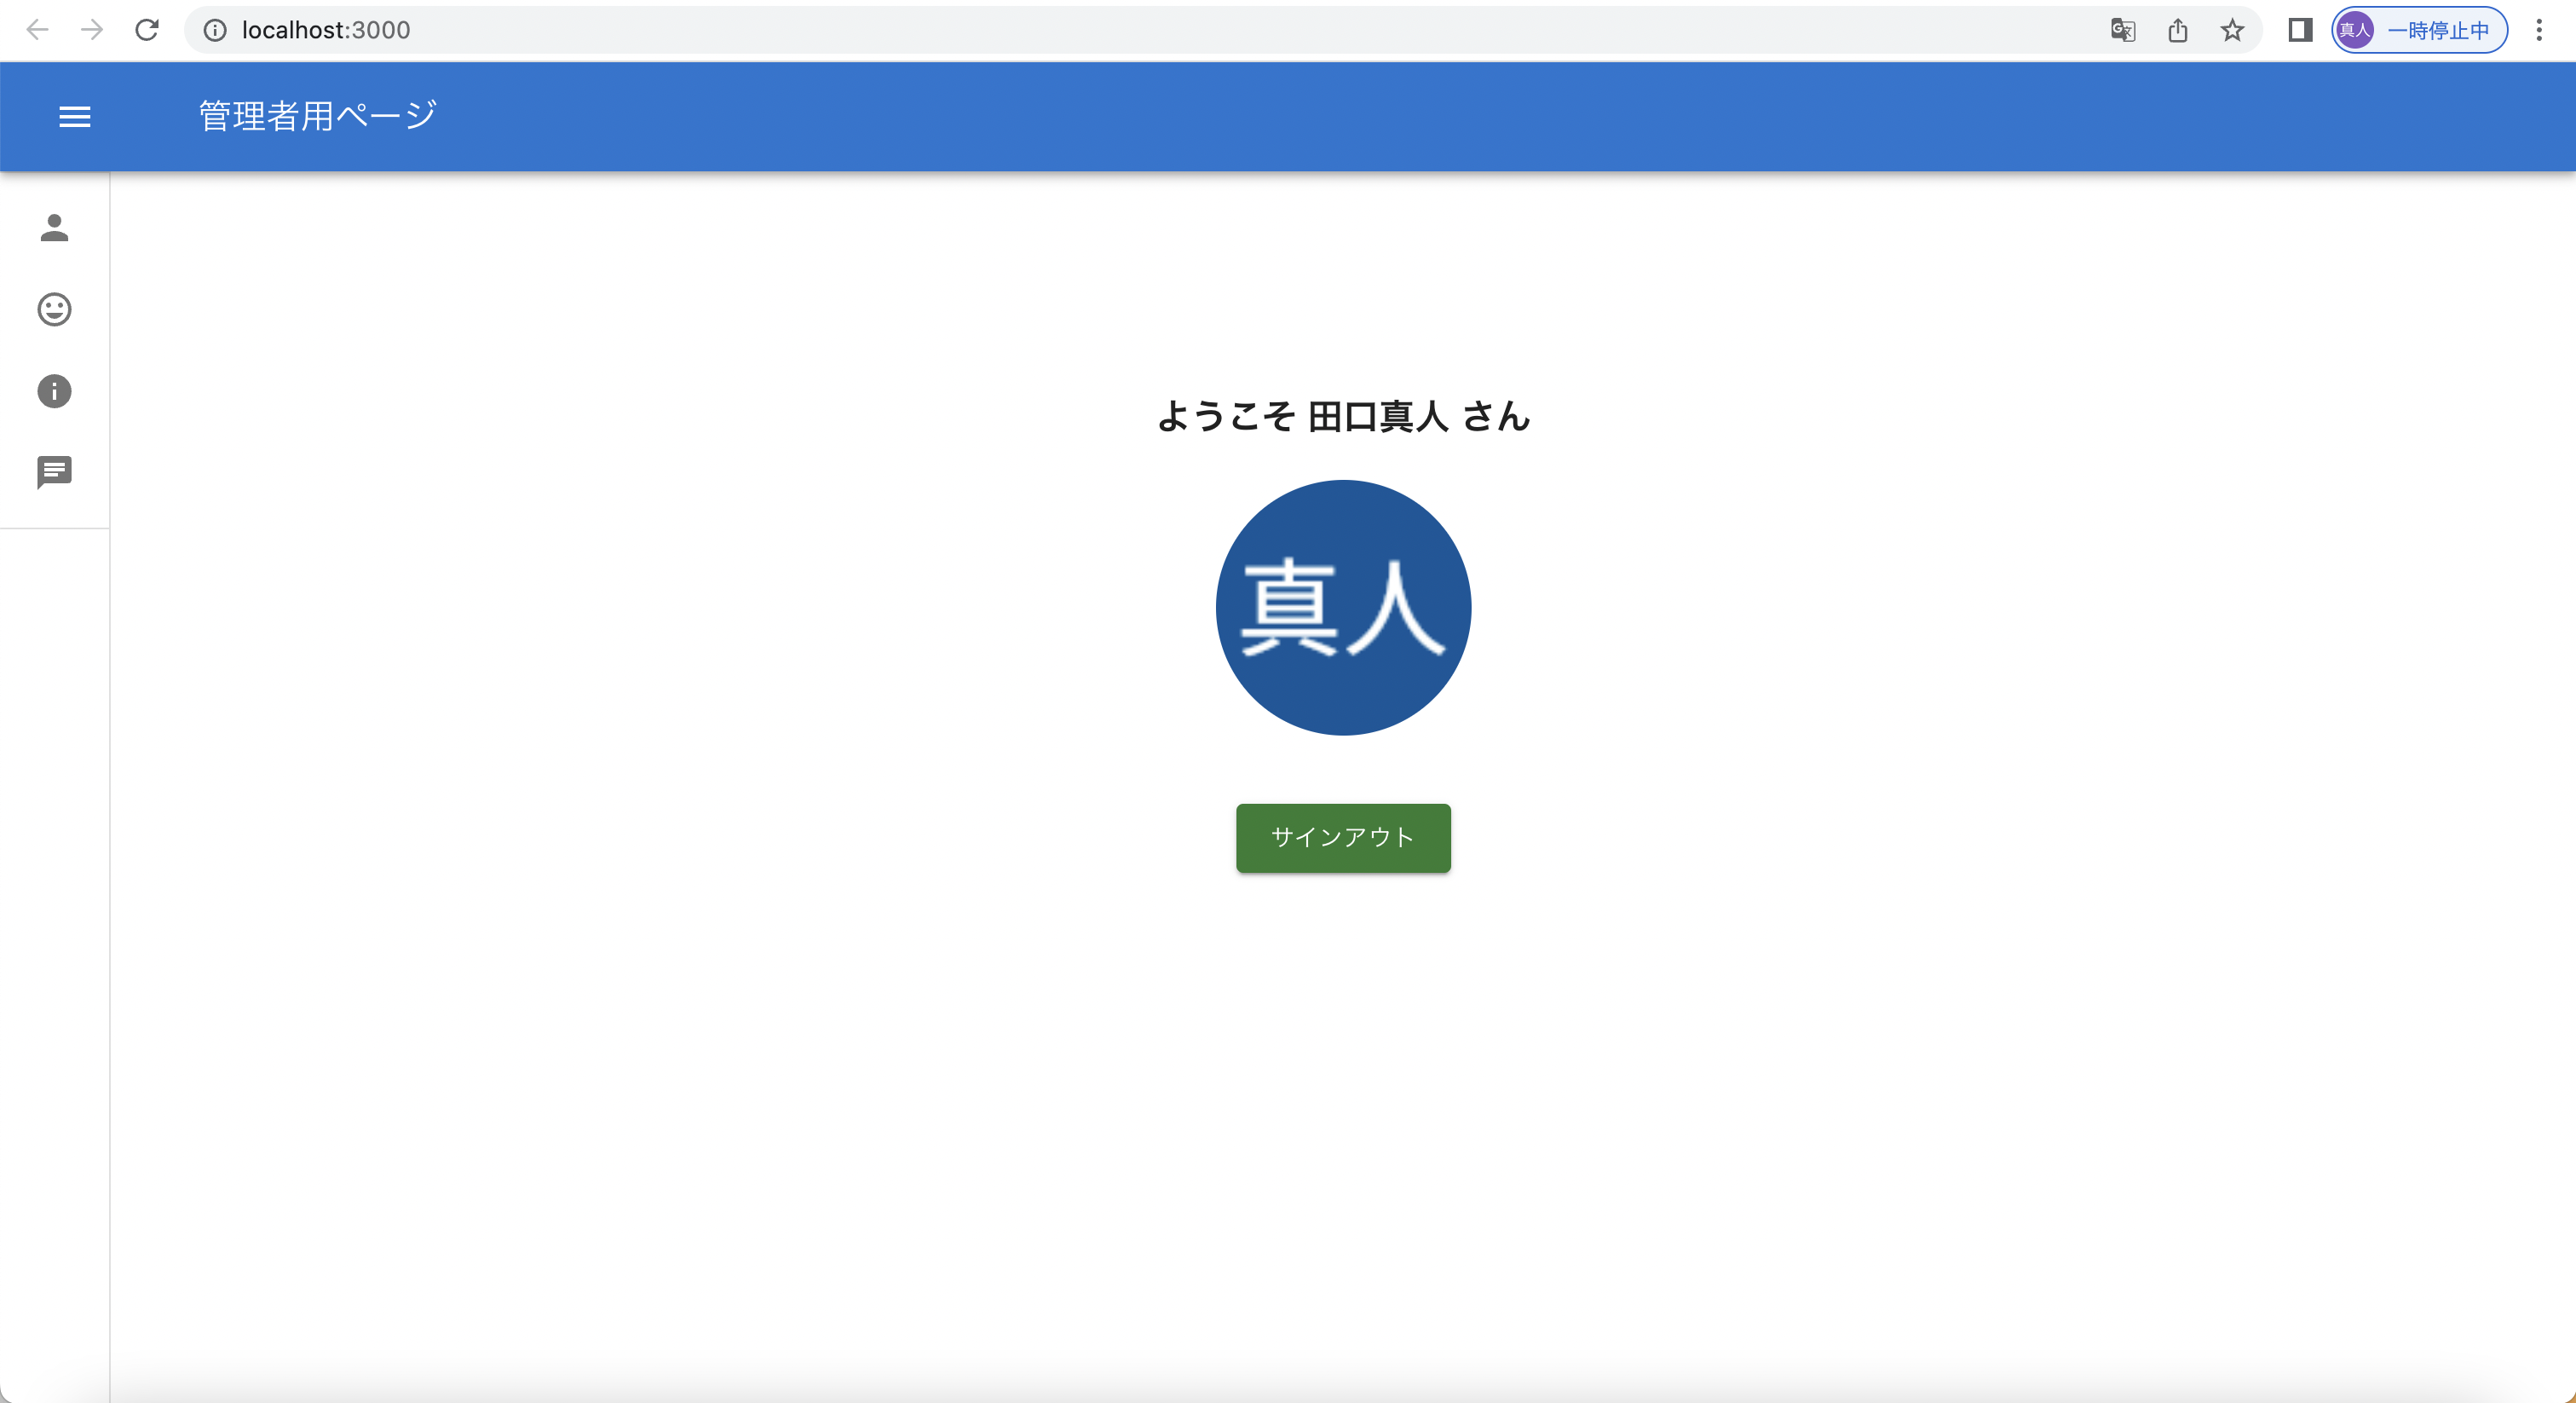
\includegraphics[scale=0.3, clip]{./img/sample15.png}
      \caption{ログイン完了画面}
      \label{fig:図の名前}
    \end{center}
    \end{figure}

    \clearpage

\section{掲示板機能}

\section{チャット機能}
